\documentclass[xcolor={dvipsnames}]{beamer} % dvipsnames gives more built-in colors
\mode<presentation>

\usetheme{Boadilla}

\definecolor{GWdarkblue}{HTML}{033C5A}

\usecolortheme[named=GWdarkblue]{structure}

% Sets the font
\usepackage[defaultfam,tabular,lining]{montserrat}
% Capital case titles
\setbeamerfont{title}{shape=\scshape}
\setbeamerfont{frametitle}{shape=\scshape}

%Remove "Figure" from captions
\setbeamertemplate{caption}{\raggedright\insertcaption\par}

\usepackage{graphicx}
\usepackage{hyperref}

\title[Data Visualization]{Data Visualization}
\author[SMPA 2152]{Data Analysis for Journalism and Political Communication (Fall 2023)}
\date{Prof. Bell}

\begin{document}


%%%%%%%%%%%%%%%%%%%%%%%%%%%%%%%%%%%%%%%%%%%%%%%%%%%%%%%%%%%%%%%%%%
\frame{
\titlepage
}

%%%%%%%%%%%%%%%%%%%%%%%%%%%%%%%%%%%%%%%%%%%%%%%%%%%%%%%%%%%%%%%%%%
\frame{
\centering
\only<1>{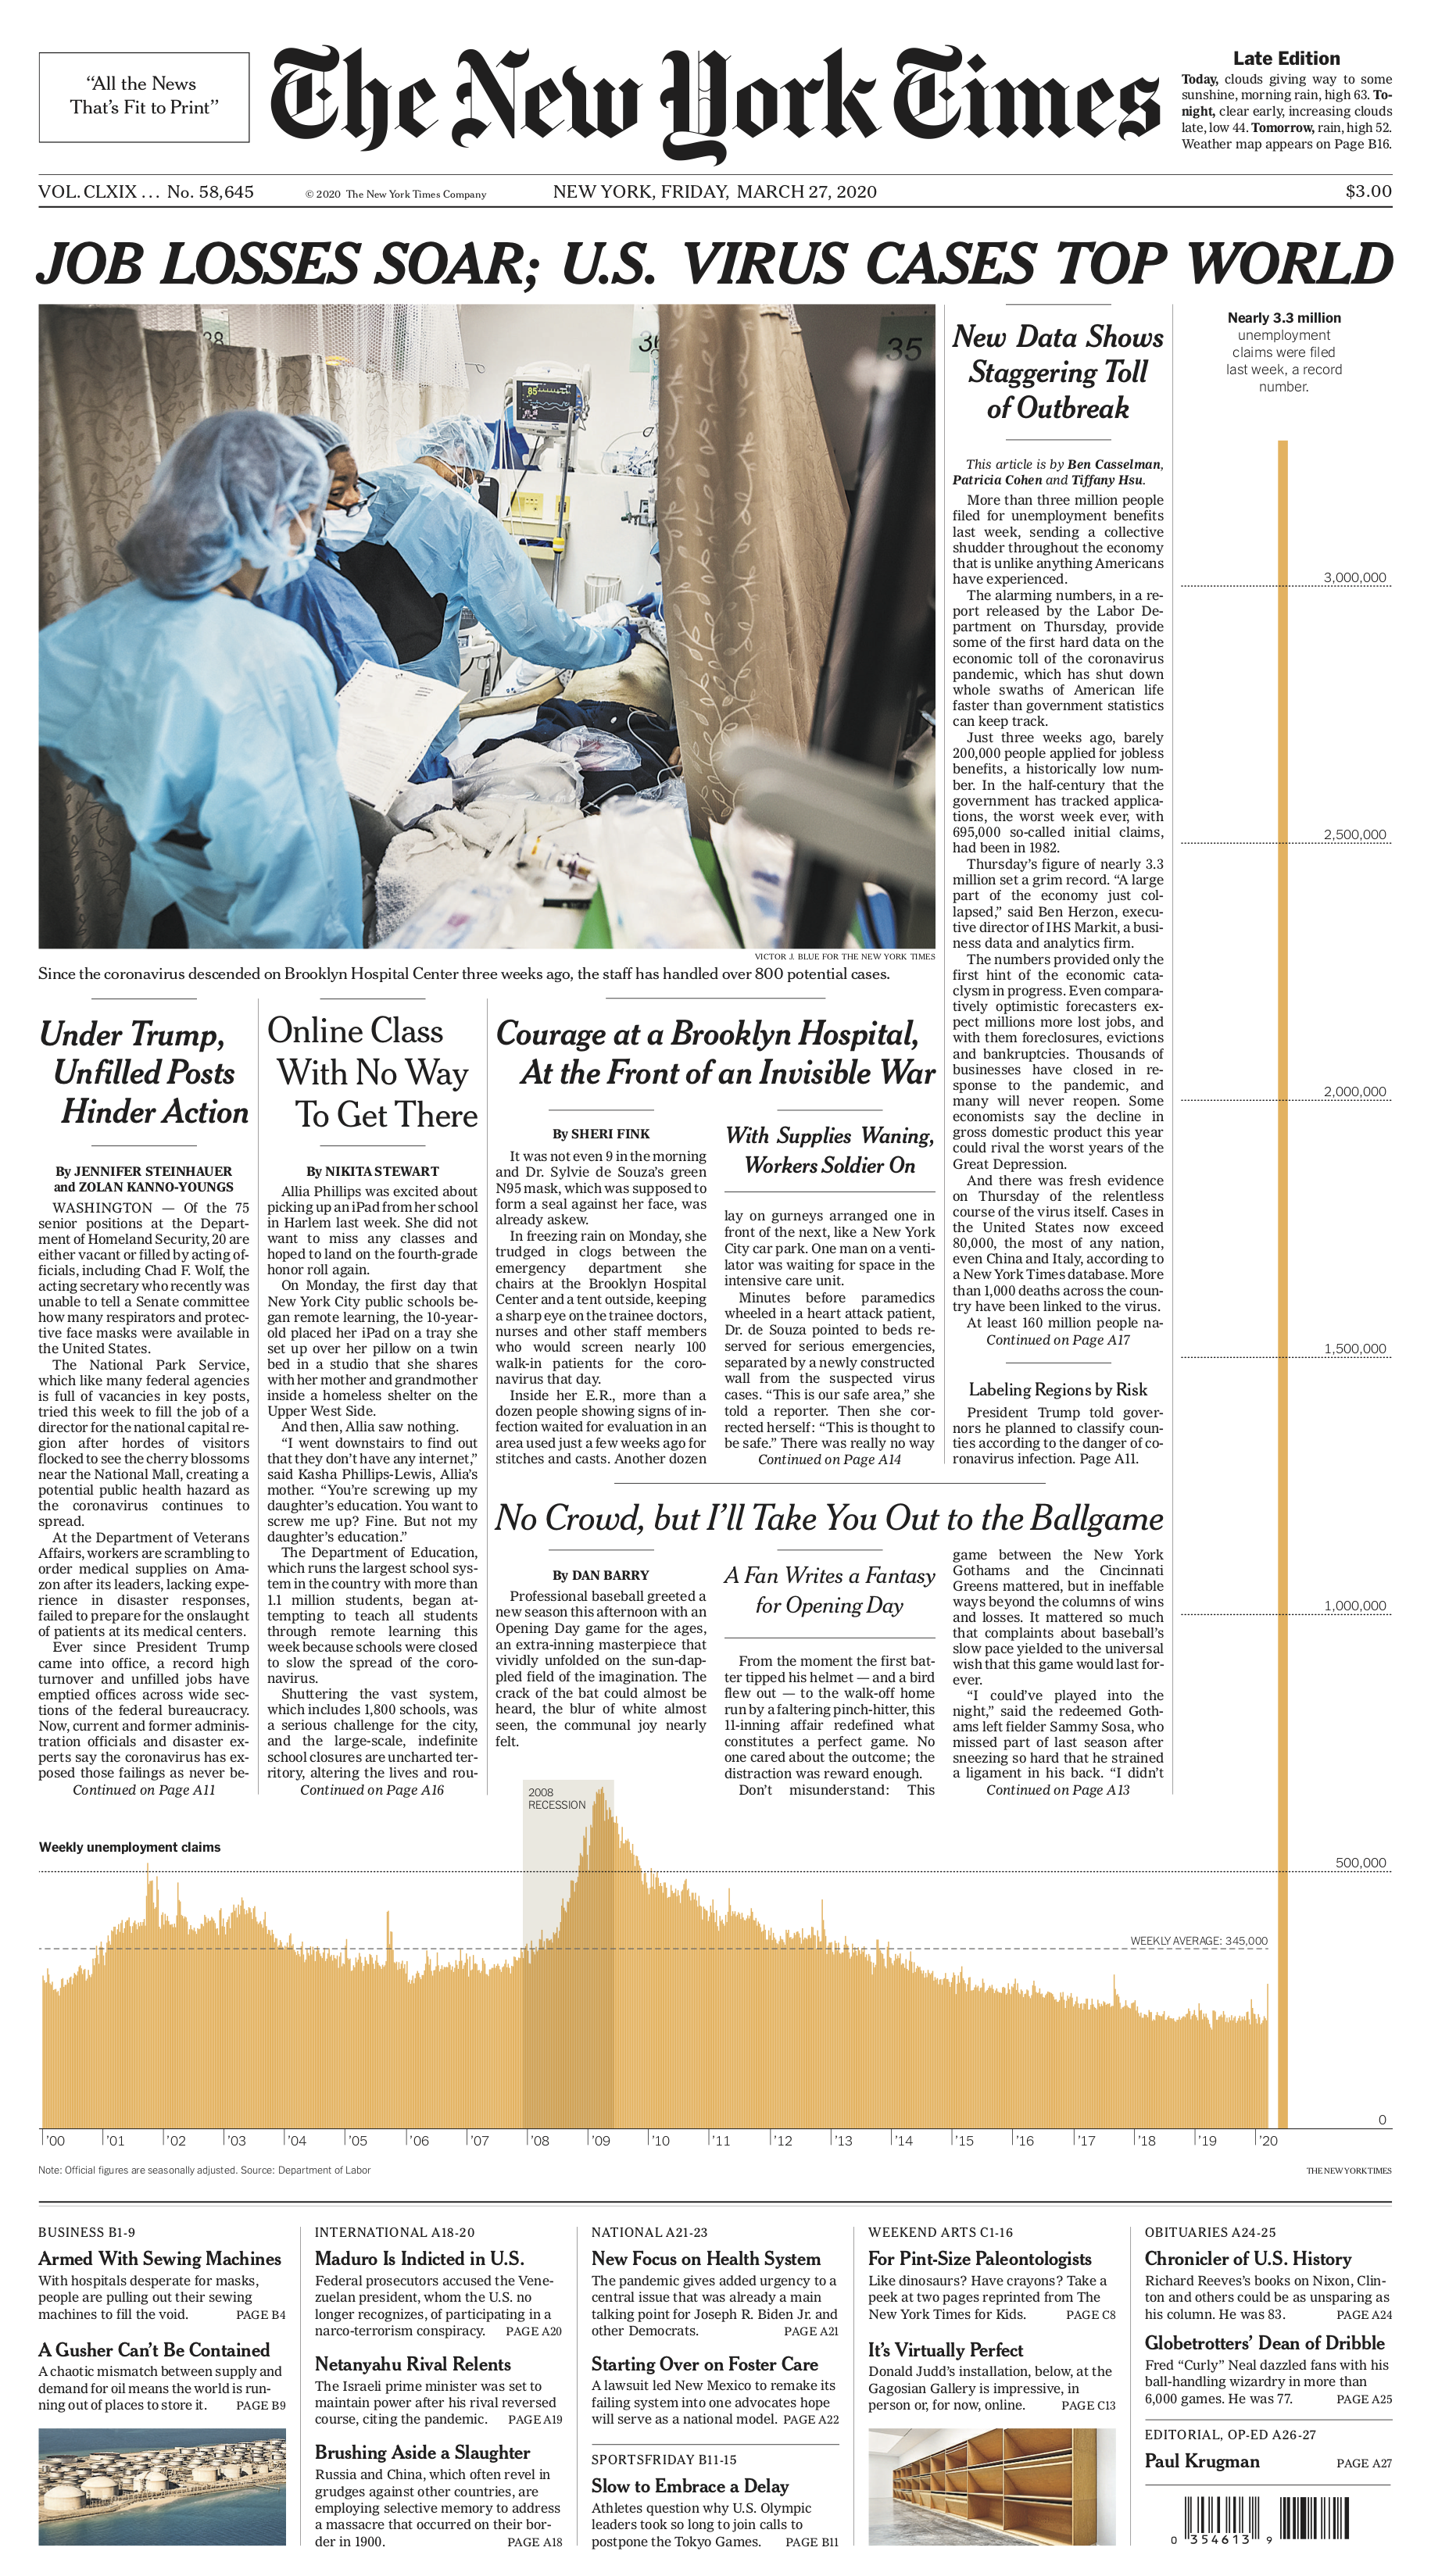
\includegraphics[height=.9\textheight]{nyt_unemp.png}}
\only<2>{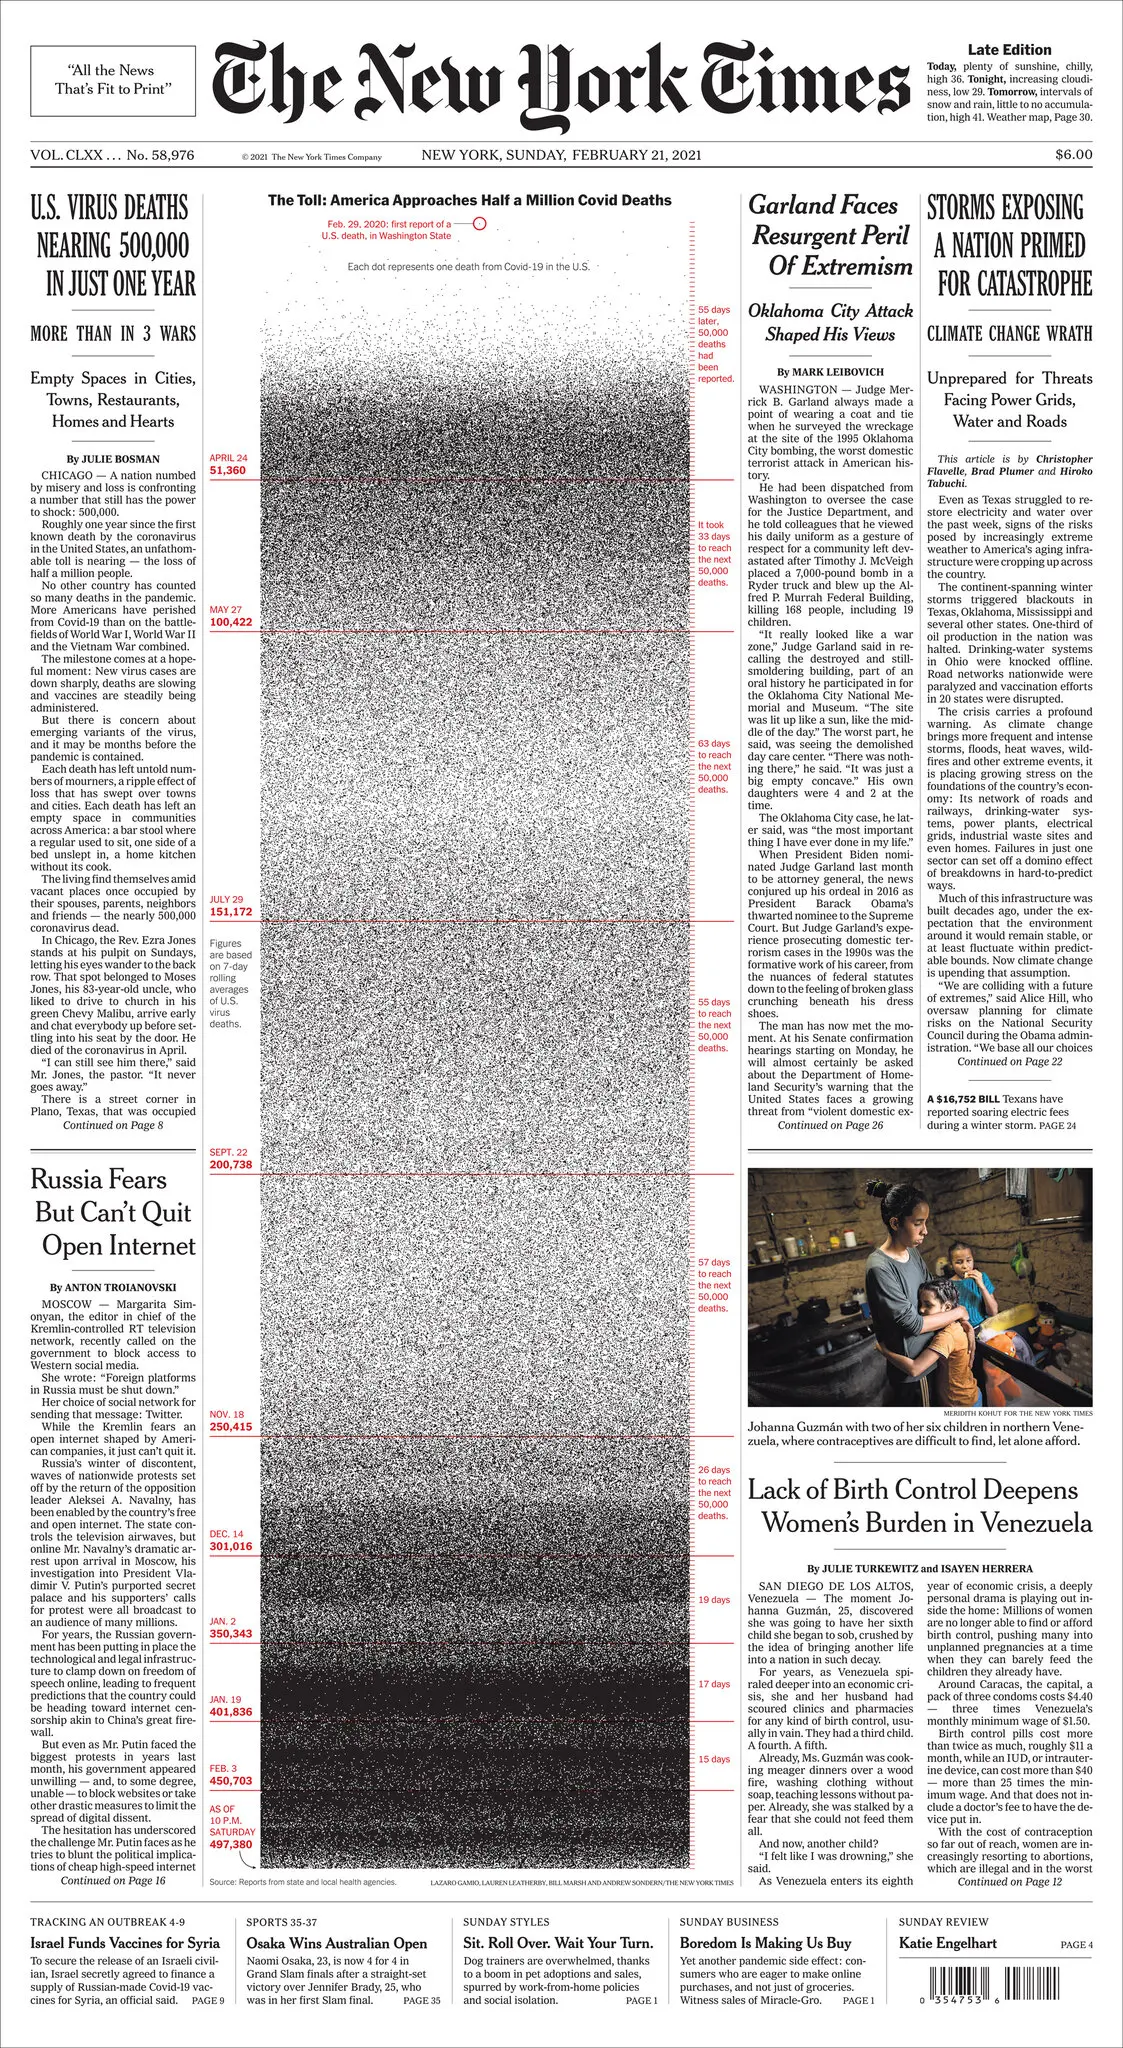
\includegraphics[height=.9\textheight]{nyt_500k.png}}
\only<3>{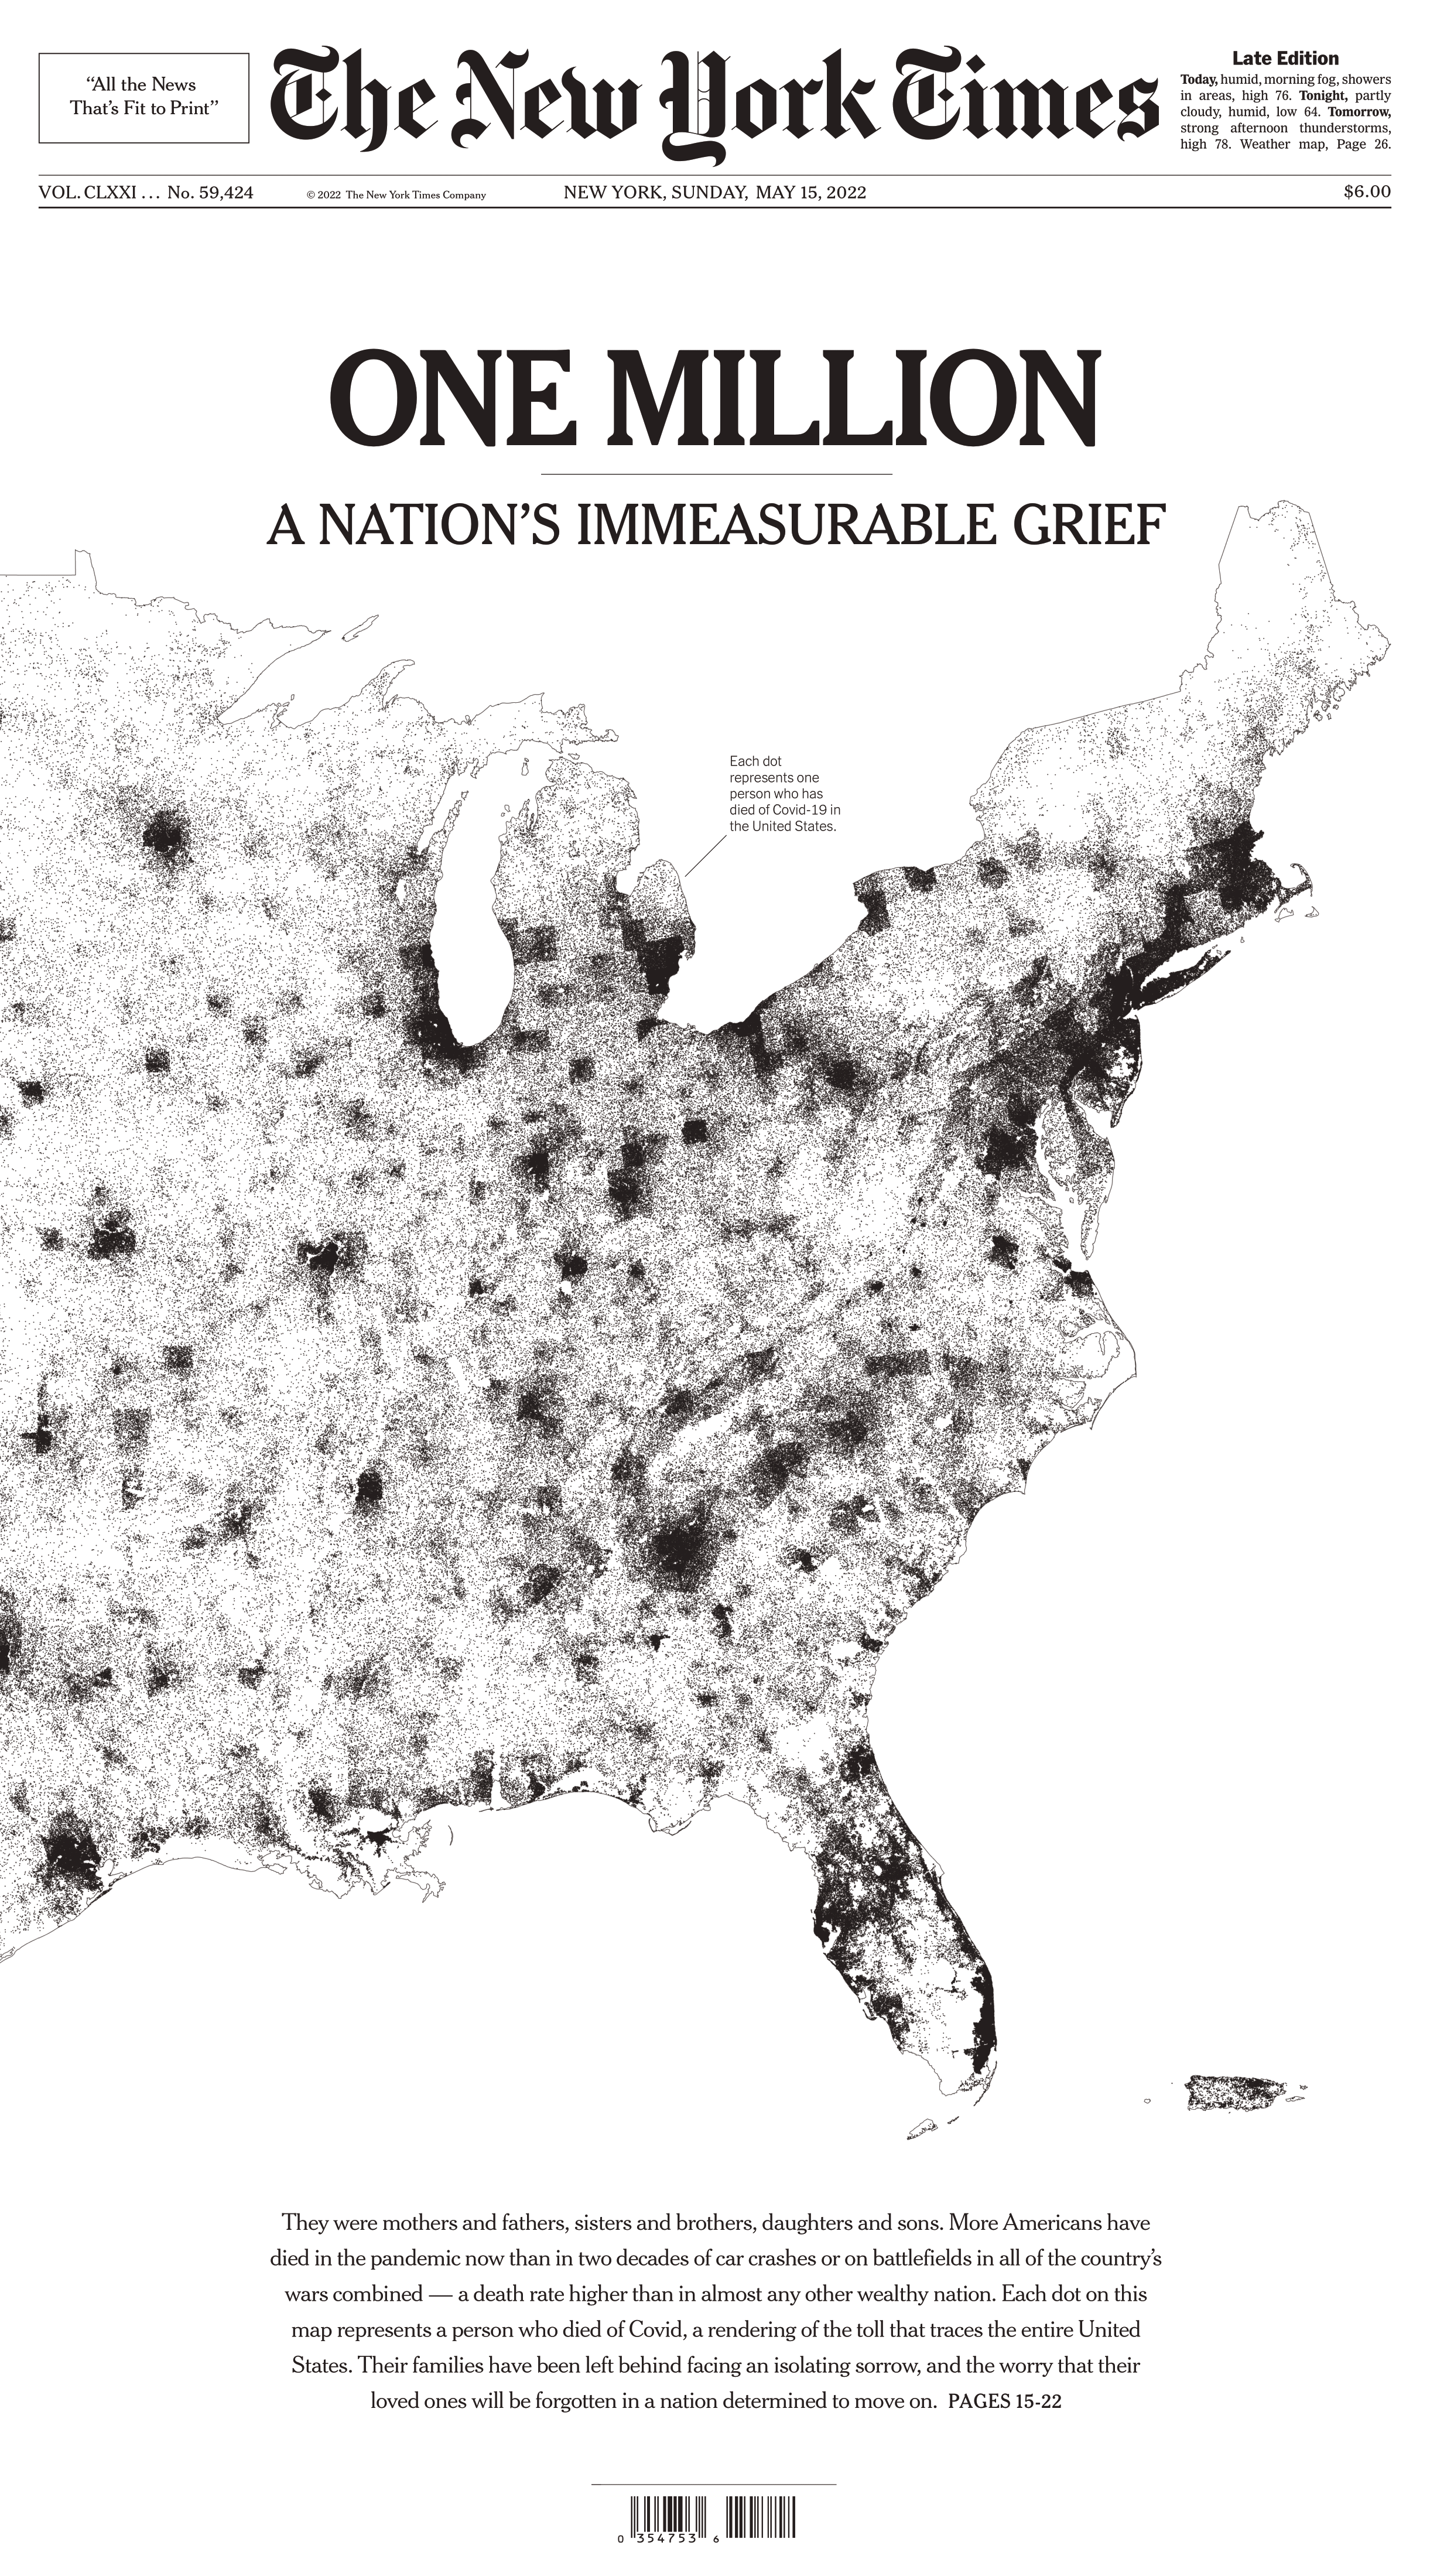
\includegraphics[height=.9\textheight]{nyt_one_million.png}}
\only<4>{
\includegraphics[height=.9\textheight]{nyt_incalculable_loss.png}}
\only<5>{
    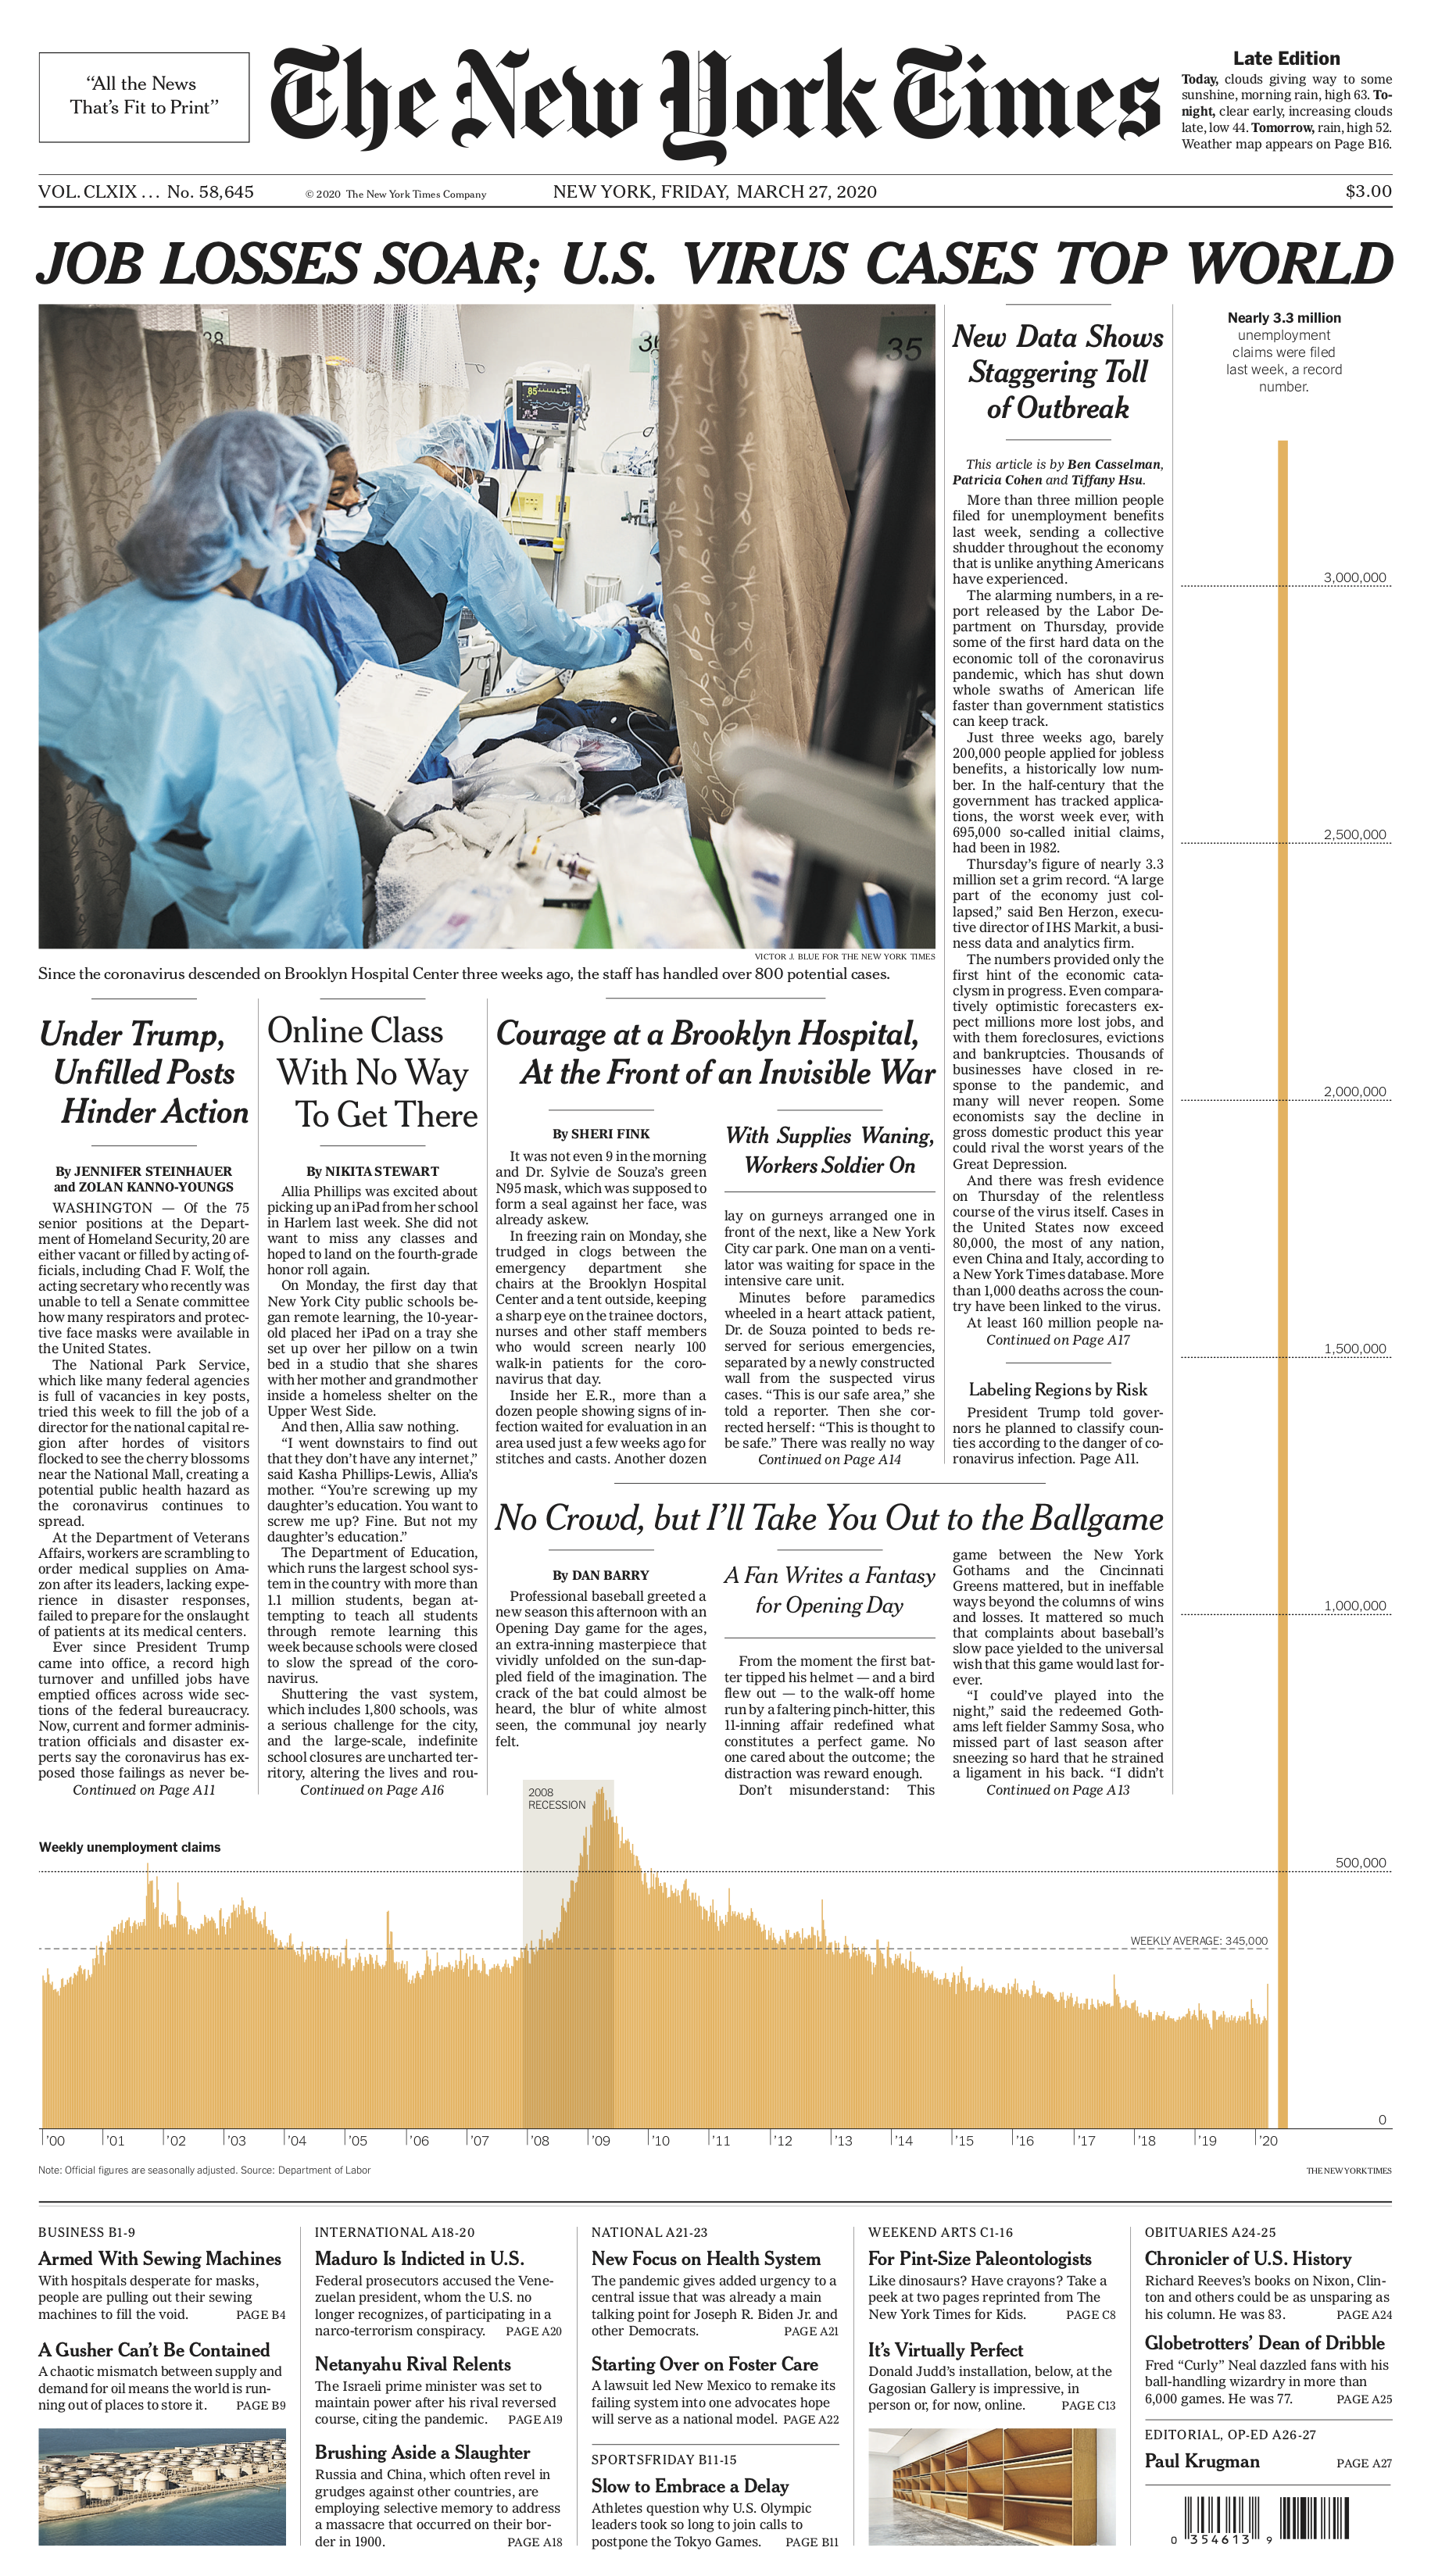
\includegraphics[width=.24\textwidth]{nyt_unemp.png} 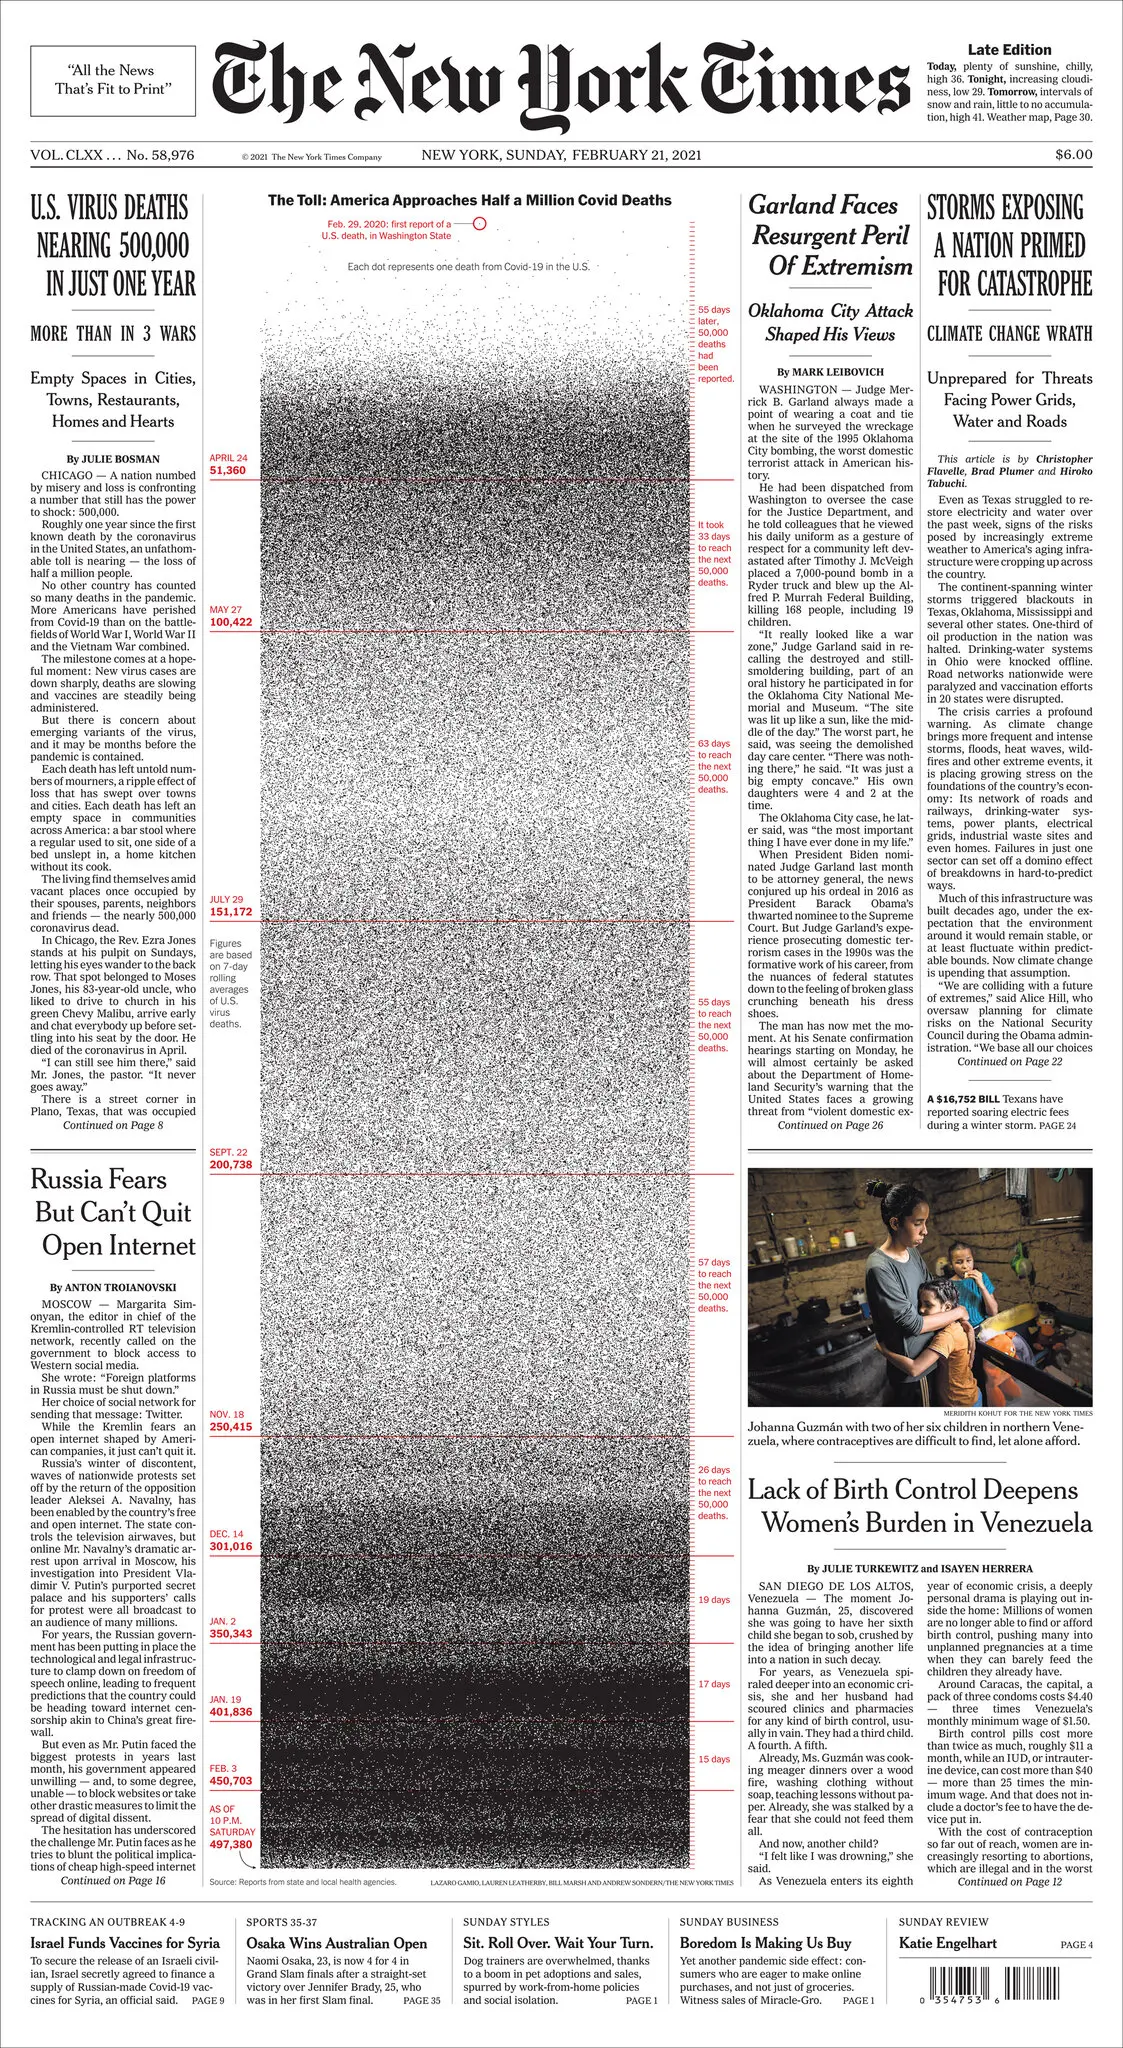
\includegraphics[width=.24\textwidth]{nyt_500k.png}
    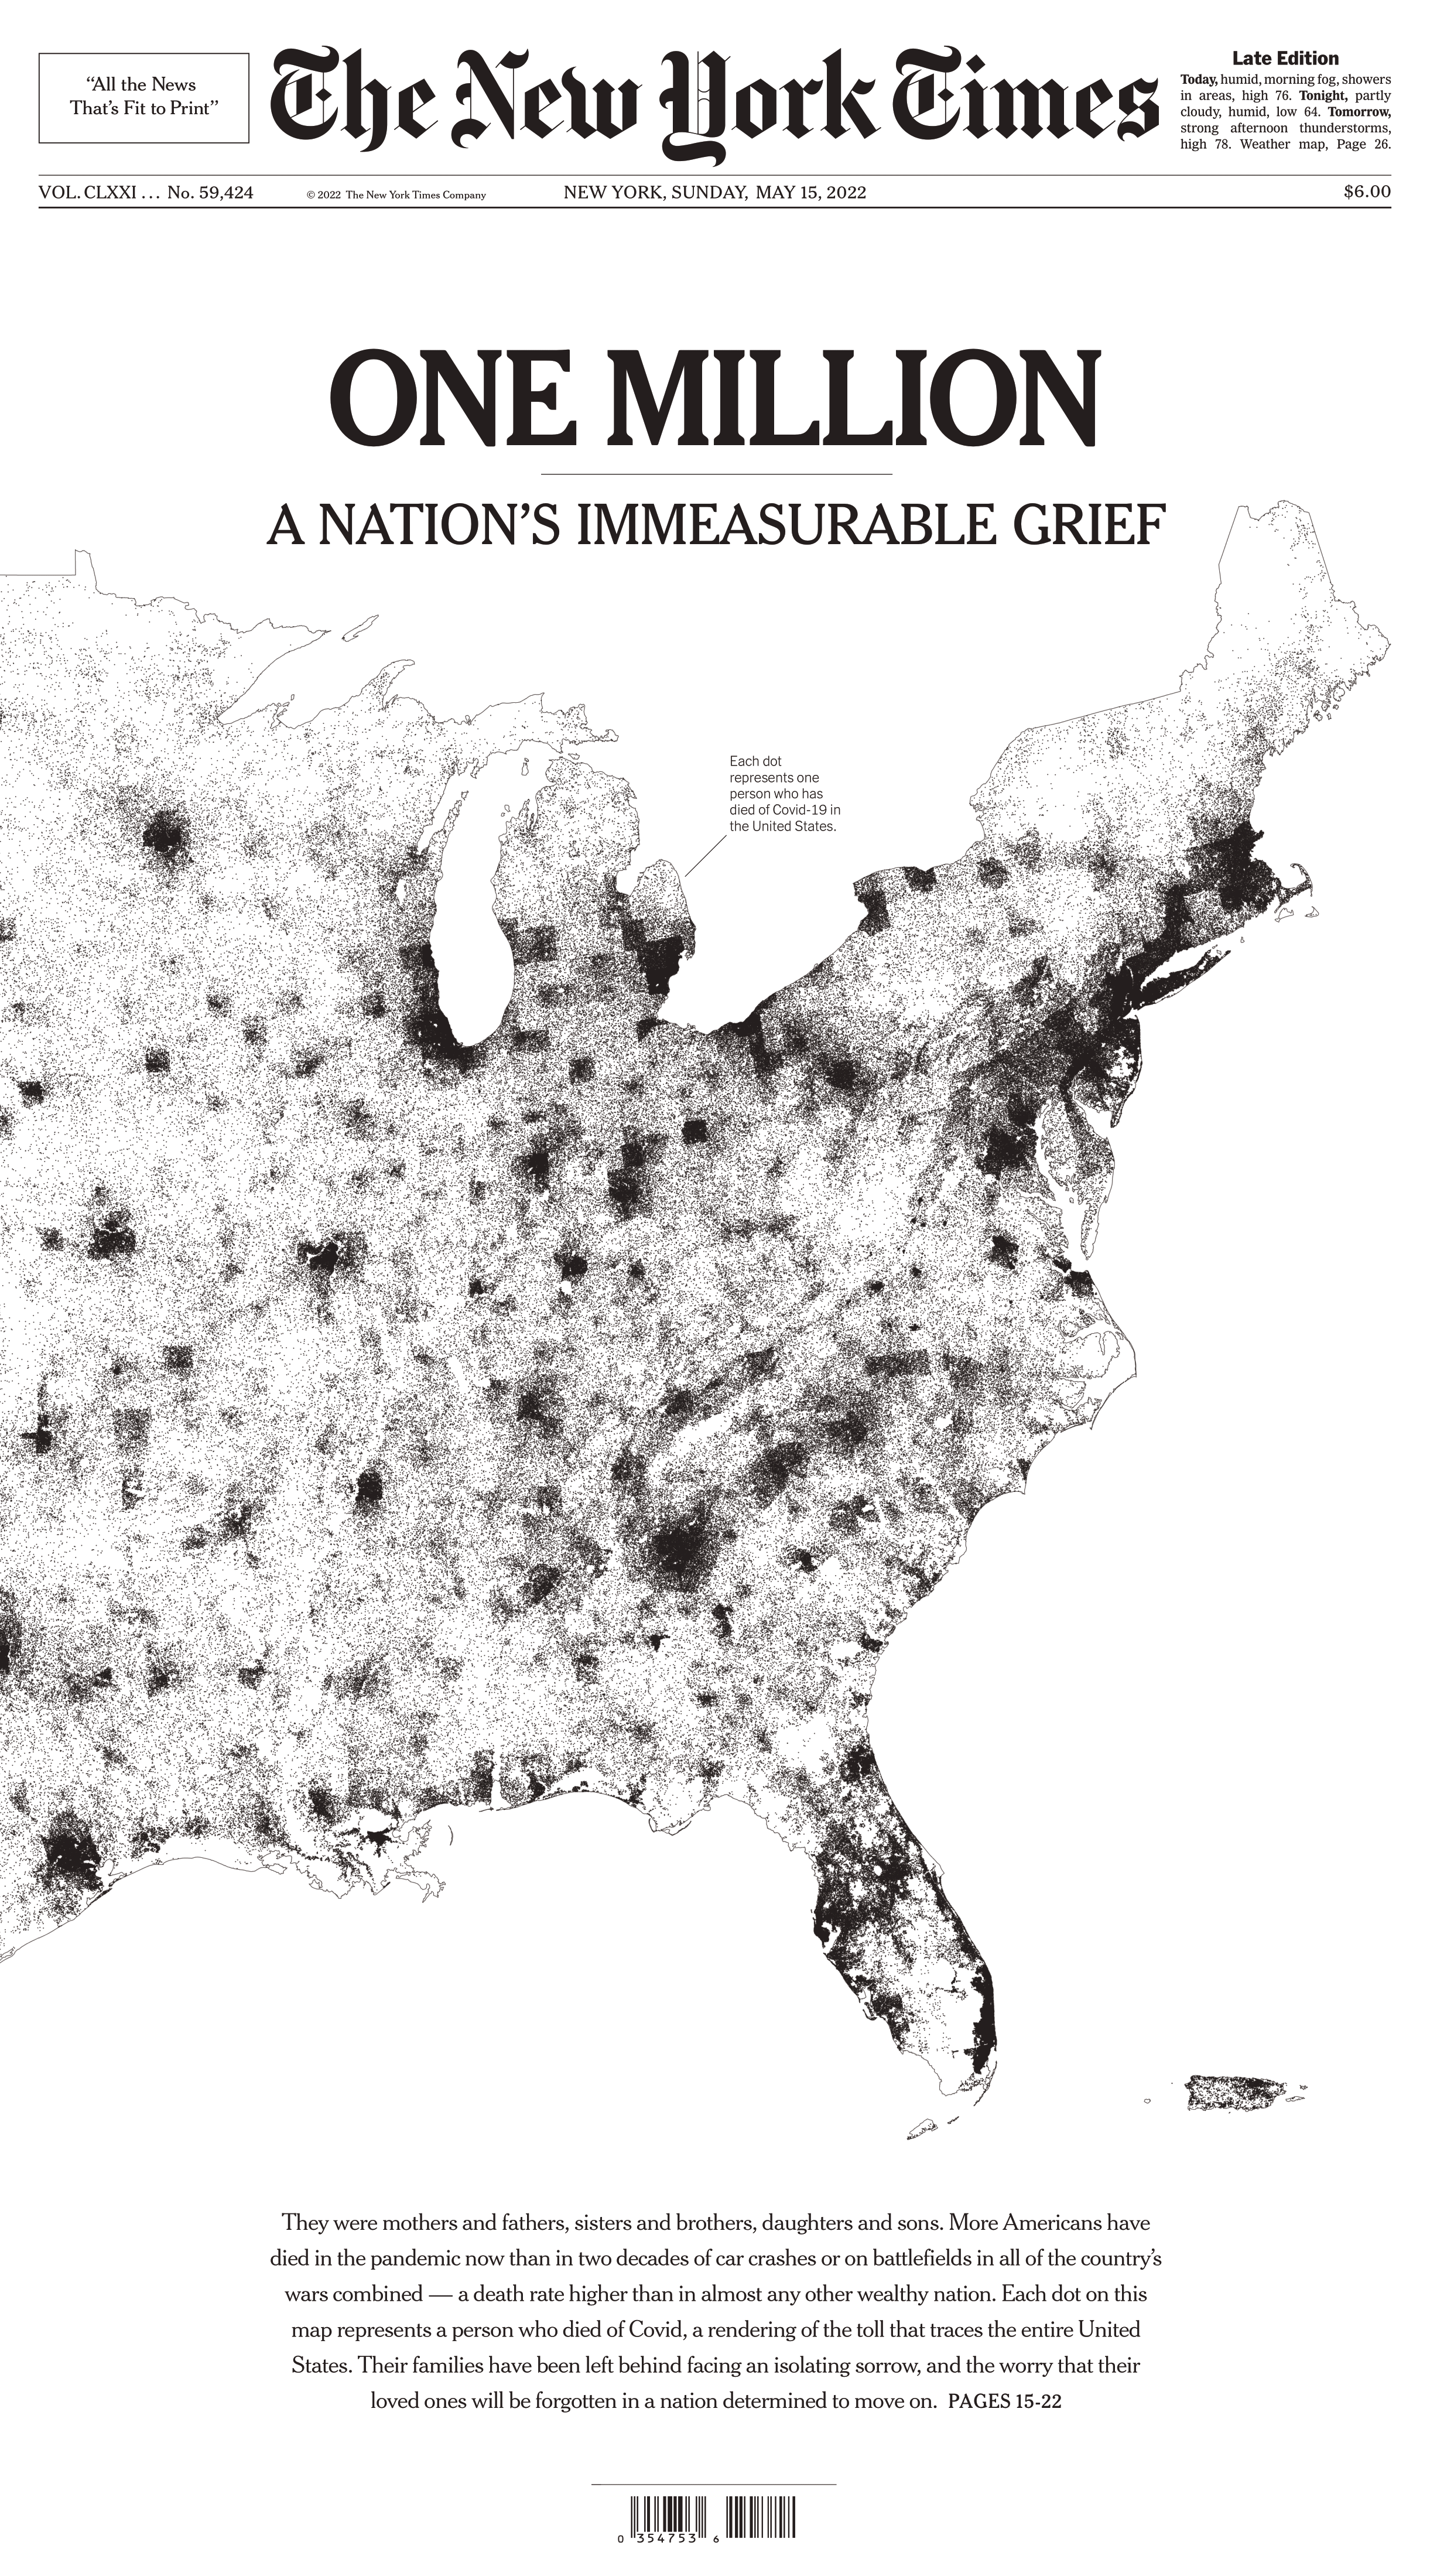
\includegraphics[width=.24\textwidth]{nyt_one_million.png} 
\includegraphics[width=.24\textwidth]{nyt_incalculable_loss.png}
}
}

%%%%%%%%%%%%%%%%%%%%%%%%%%%%%%%%%%%%%%%%%%%%%%%%%%%%%%%%%%%%%%%%%%
\frame{\frametitle{Early Data Visualization}
\only<1>{
    \centering
    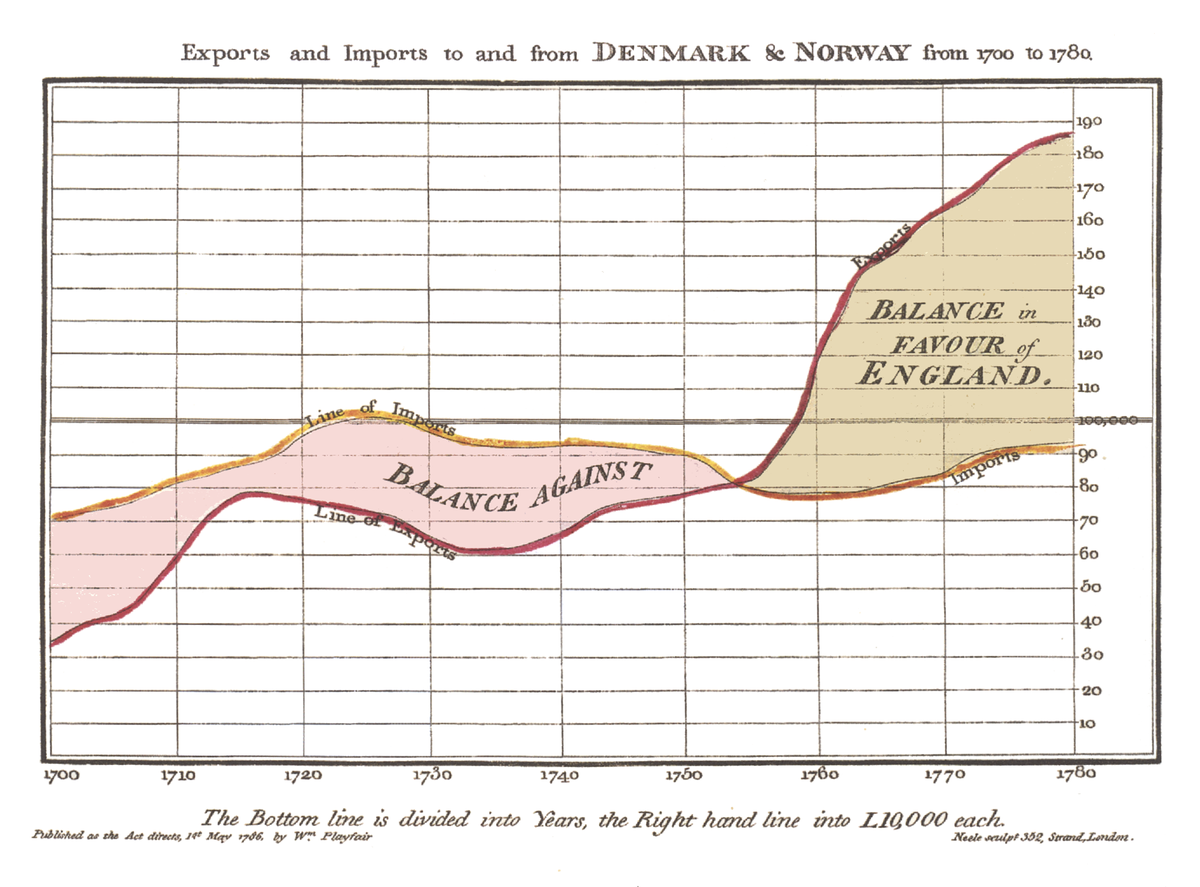
\includegraphics[height=.75\textheight]{Playfair.png}\\
    William Playfair (late 1700s)
}
\only<2>{
    \centering
    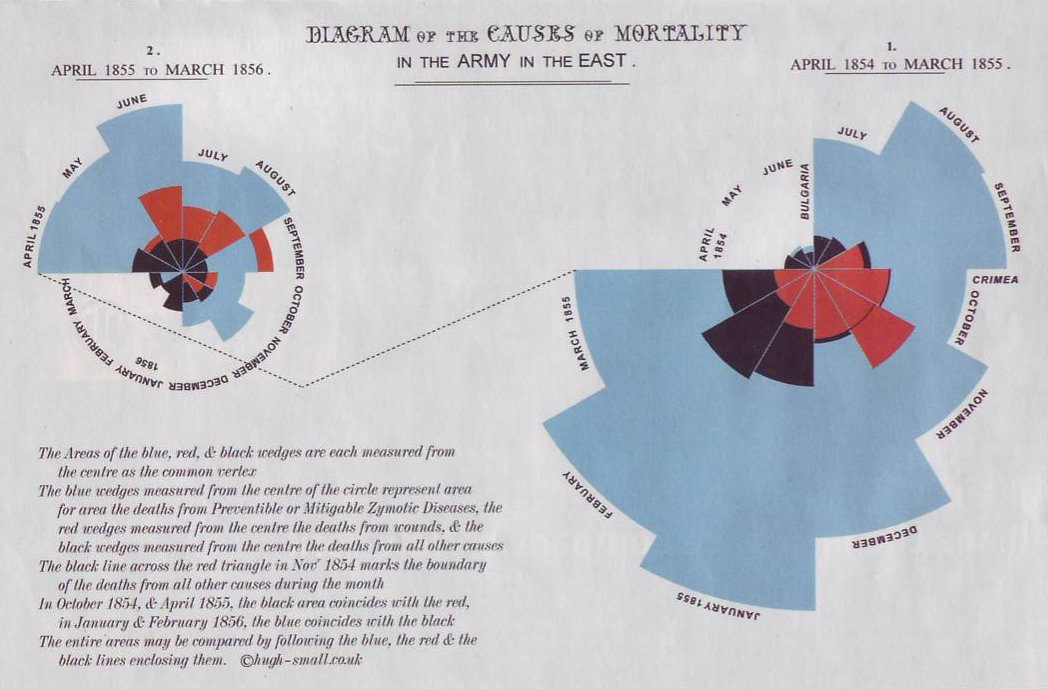
\includegraphics[height=.75\textheight]{Nightingale.jpg}\\
    Florence Nightingale (1858)
}
\only<3>{
    \centering
    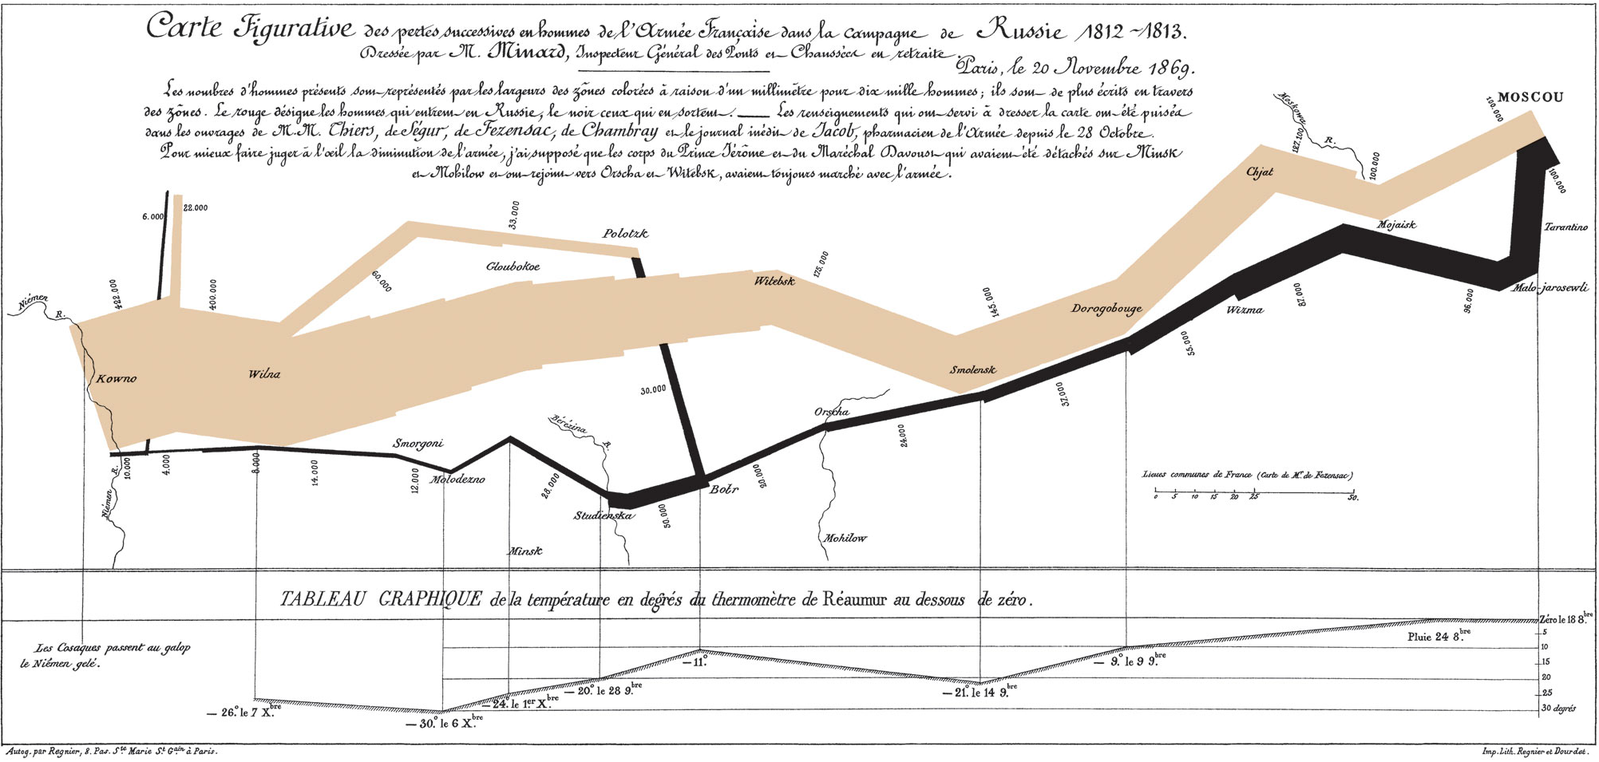
\includegraphics[width=\textwidth]{Minard.png}\\
    Charles Minard (1861)
}
}

%%%%%%%%%%%%%%%%%%%%%%%%%%%%%%%%%%%%%%%%%%%%%%%%%%%%%%%%%%%%%%%%%%
\frame{\frametitle{Modern Day: The Tufte Graph}
\centering
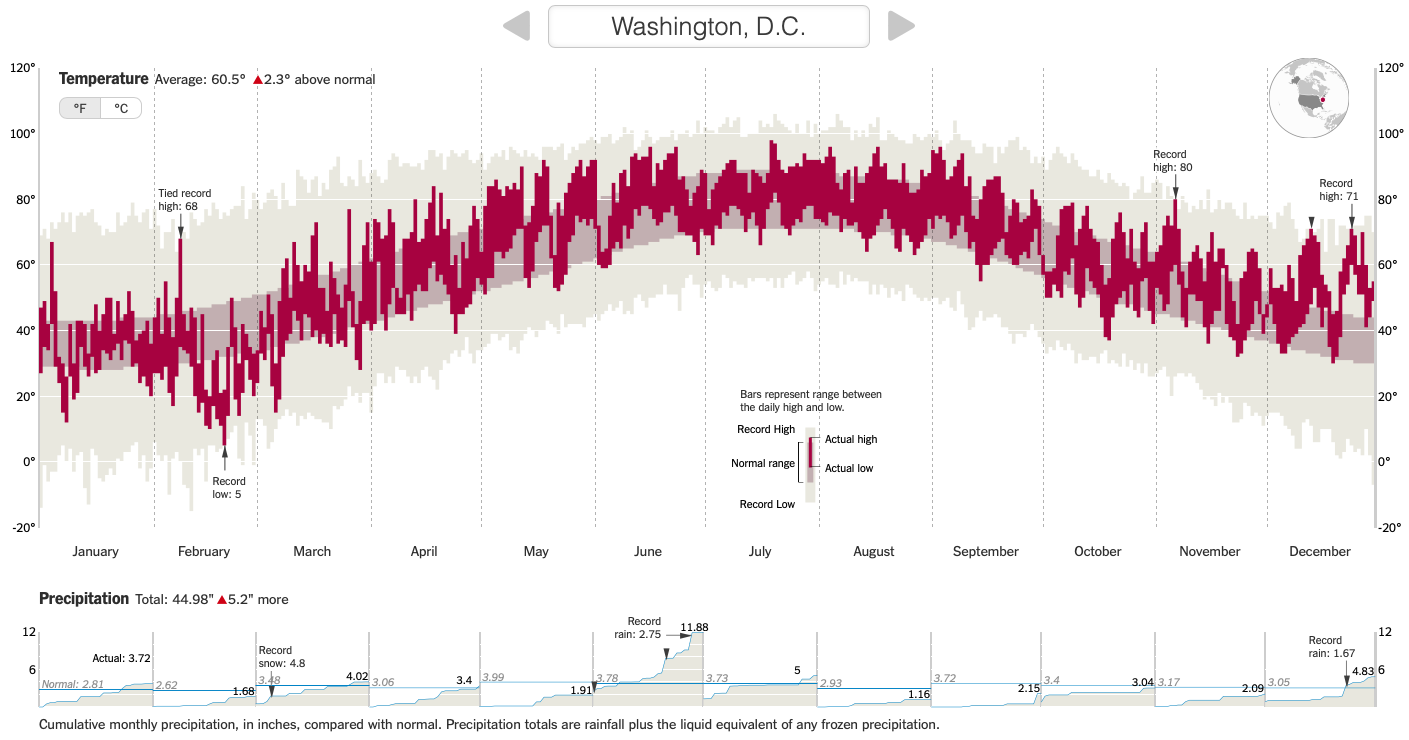
\includegraphics[width=\textwidth]{Tufte.png}
\begin{block}{}
    \centering
    ``Above all else, show the data.'' - Edward Tufte
\end{block}
}

%%%%%%%%%%%%%%%%%%%%%%%%%%%%%%%%%%%%%%%%%%%%%%%%%%%%%%%%%%%%%%%%%%
\frame{\frametitle{Art and Science of Visualization}
\only<1>{
    \centering
    \href{https://bookshop.org/books/good-charts-the-hbr-guide-to-making-smarter-more-persuasive-data-visualizations/9781633690707}{
    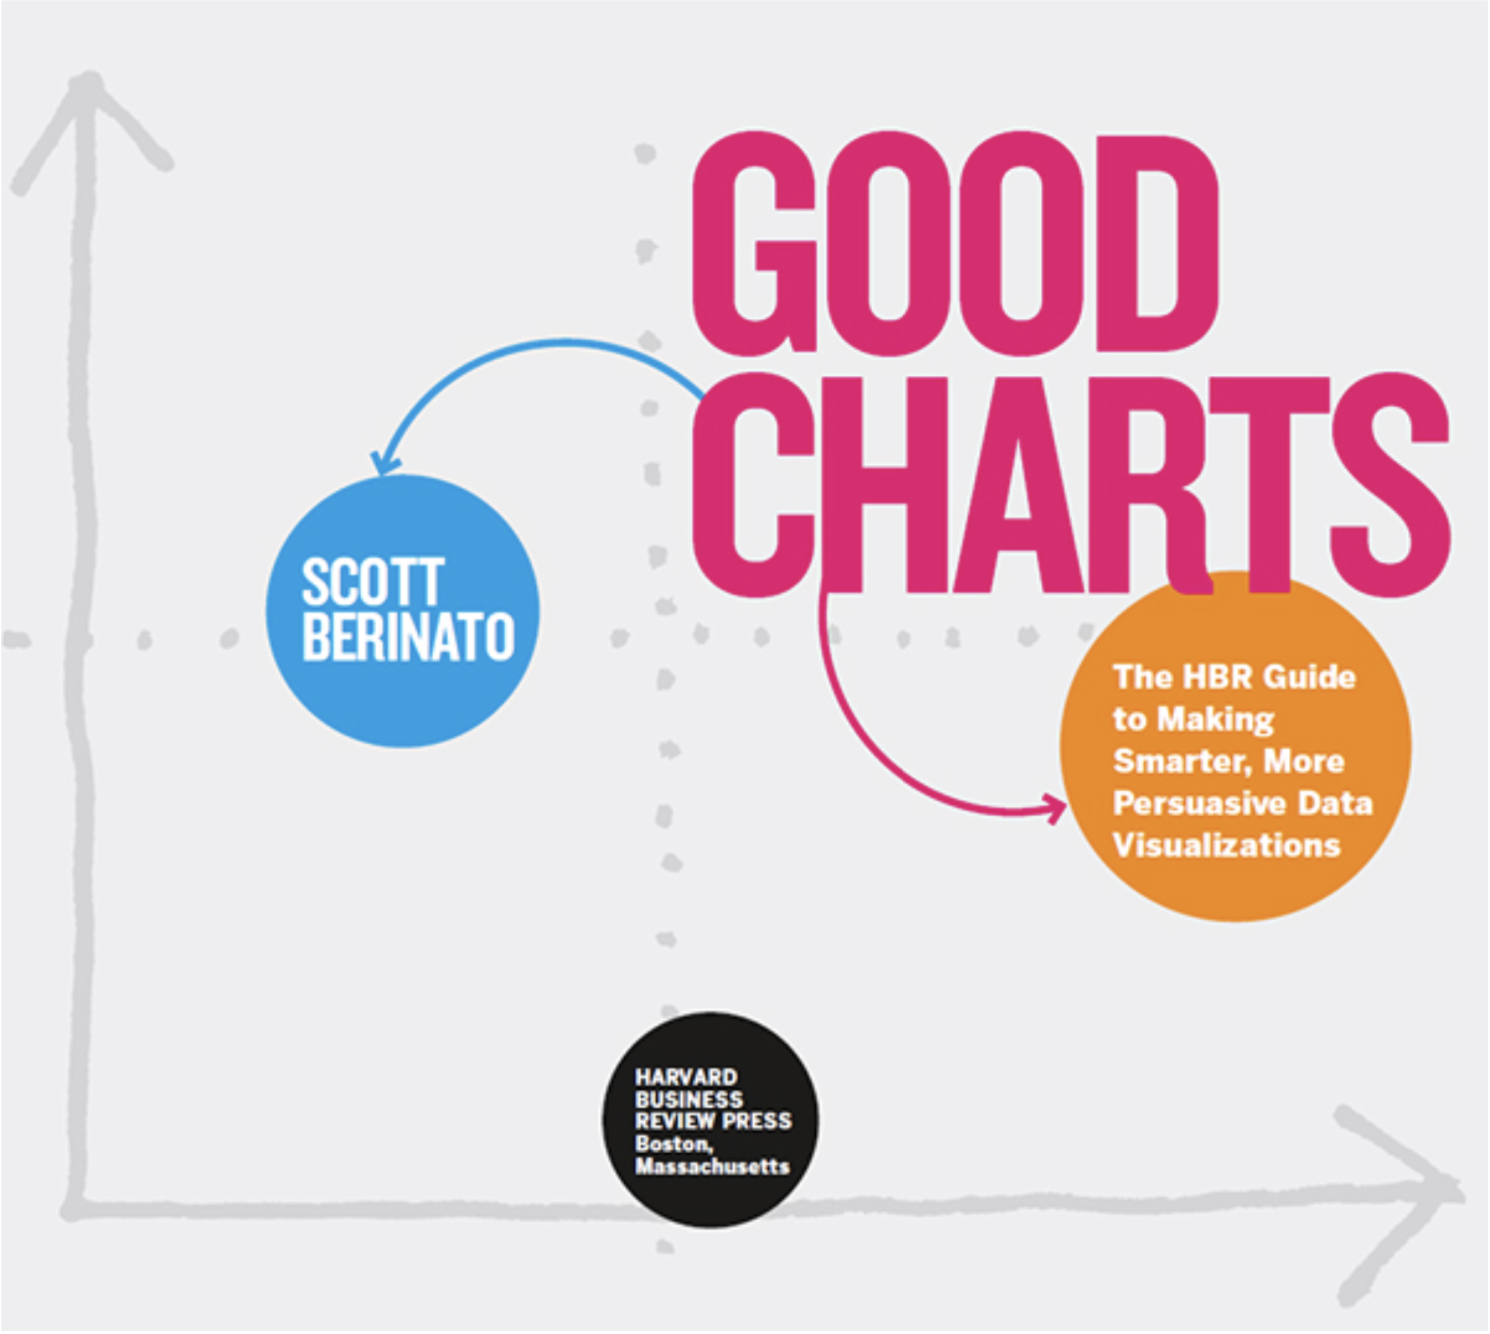
\includegraphics[height=.8\textheight]{berinato.png}}
}
\only<2->{
\begin{columns}
    \column{0.4\textwidth}
    \begin{enumerate}[<+(1)->]
            \item We don't always go in order
            \item<4-> We see first what stands out
            \item<6-> We only see a few things at once
            \item<8-> We seek meaning and make connections
            \item<10-> We rely on conventions and metaphors
        \end{enumerate}
    \column{0.6\textwidth}
    \centering
    \only<2>{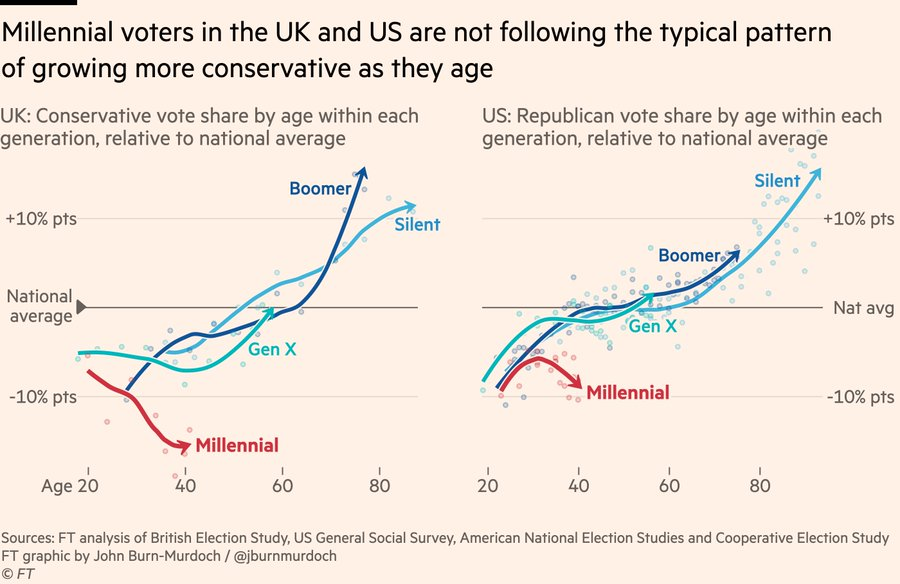
\includegraphics[width=\textwidth]{ft_partisanship.png}}
    \only<3>{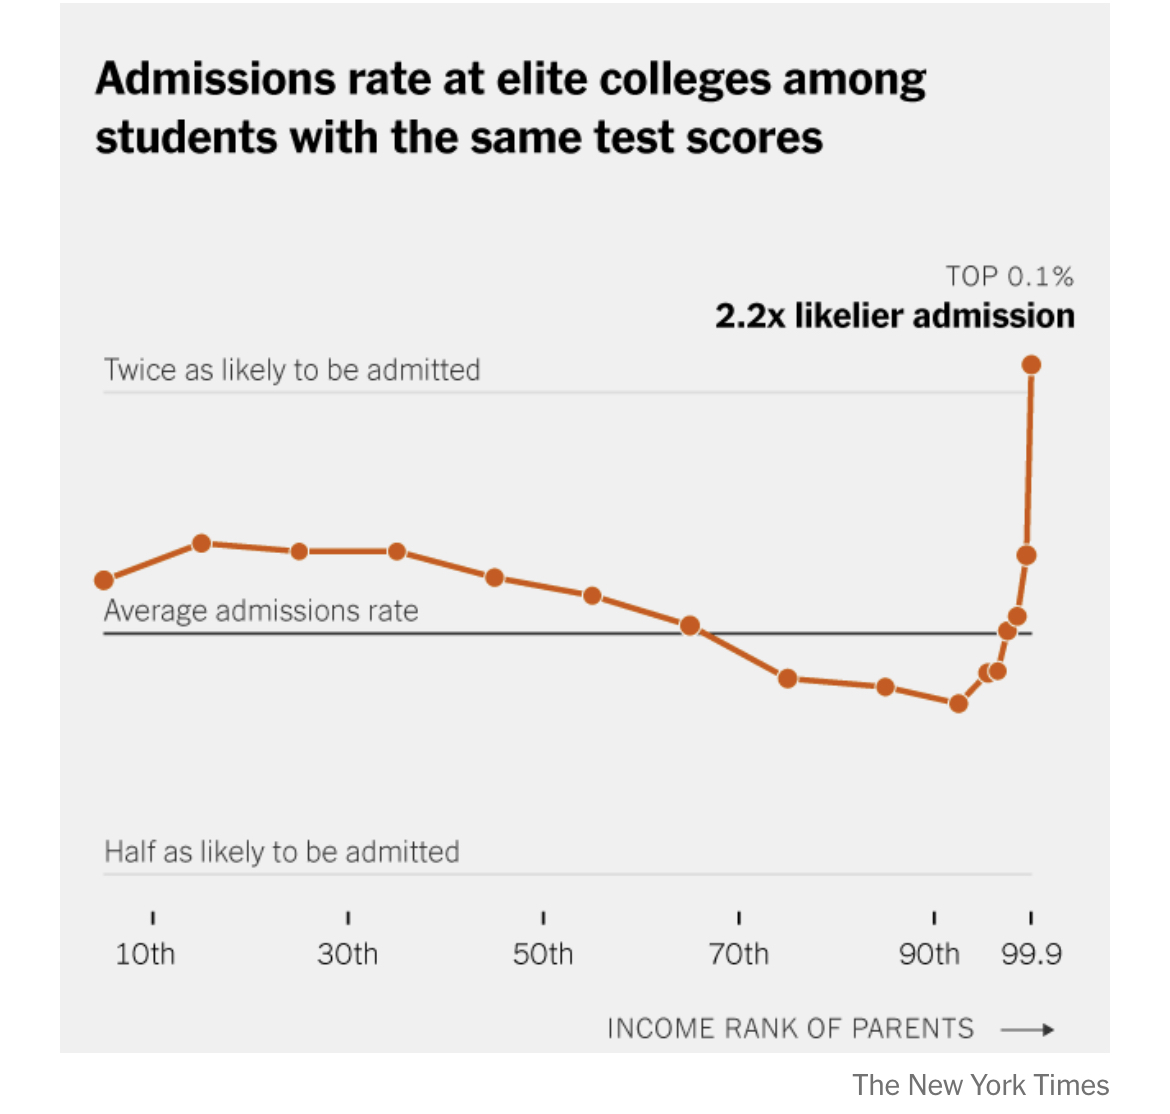
\includegraphics[width=\textwidth]{nyt_admissions.jpg}}
    \only<4>{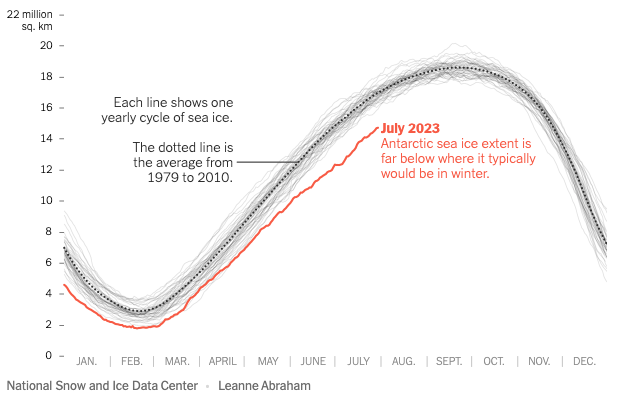
\includegraphics[width=\textwidth]{nyt_antarctic_ice.png}}
    \only<5>{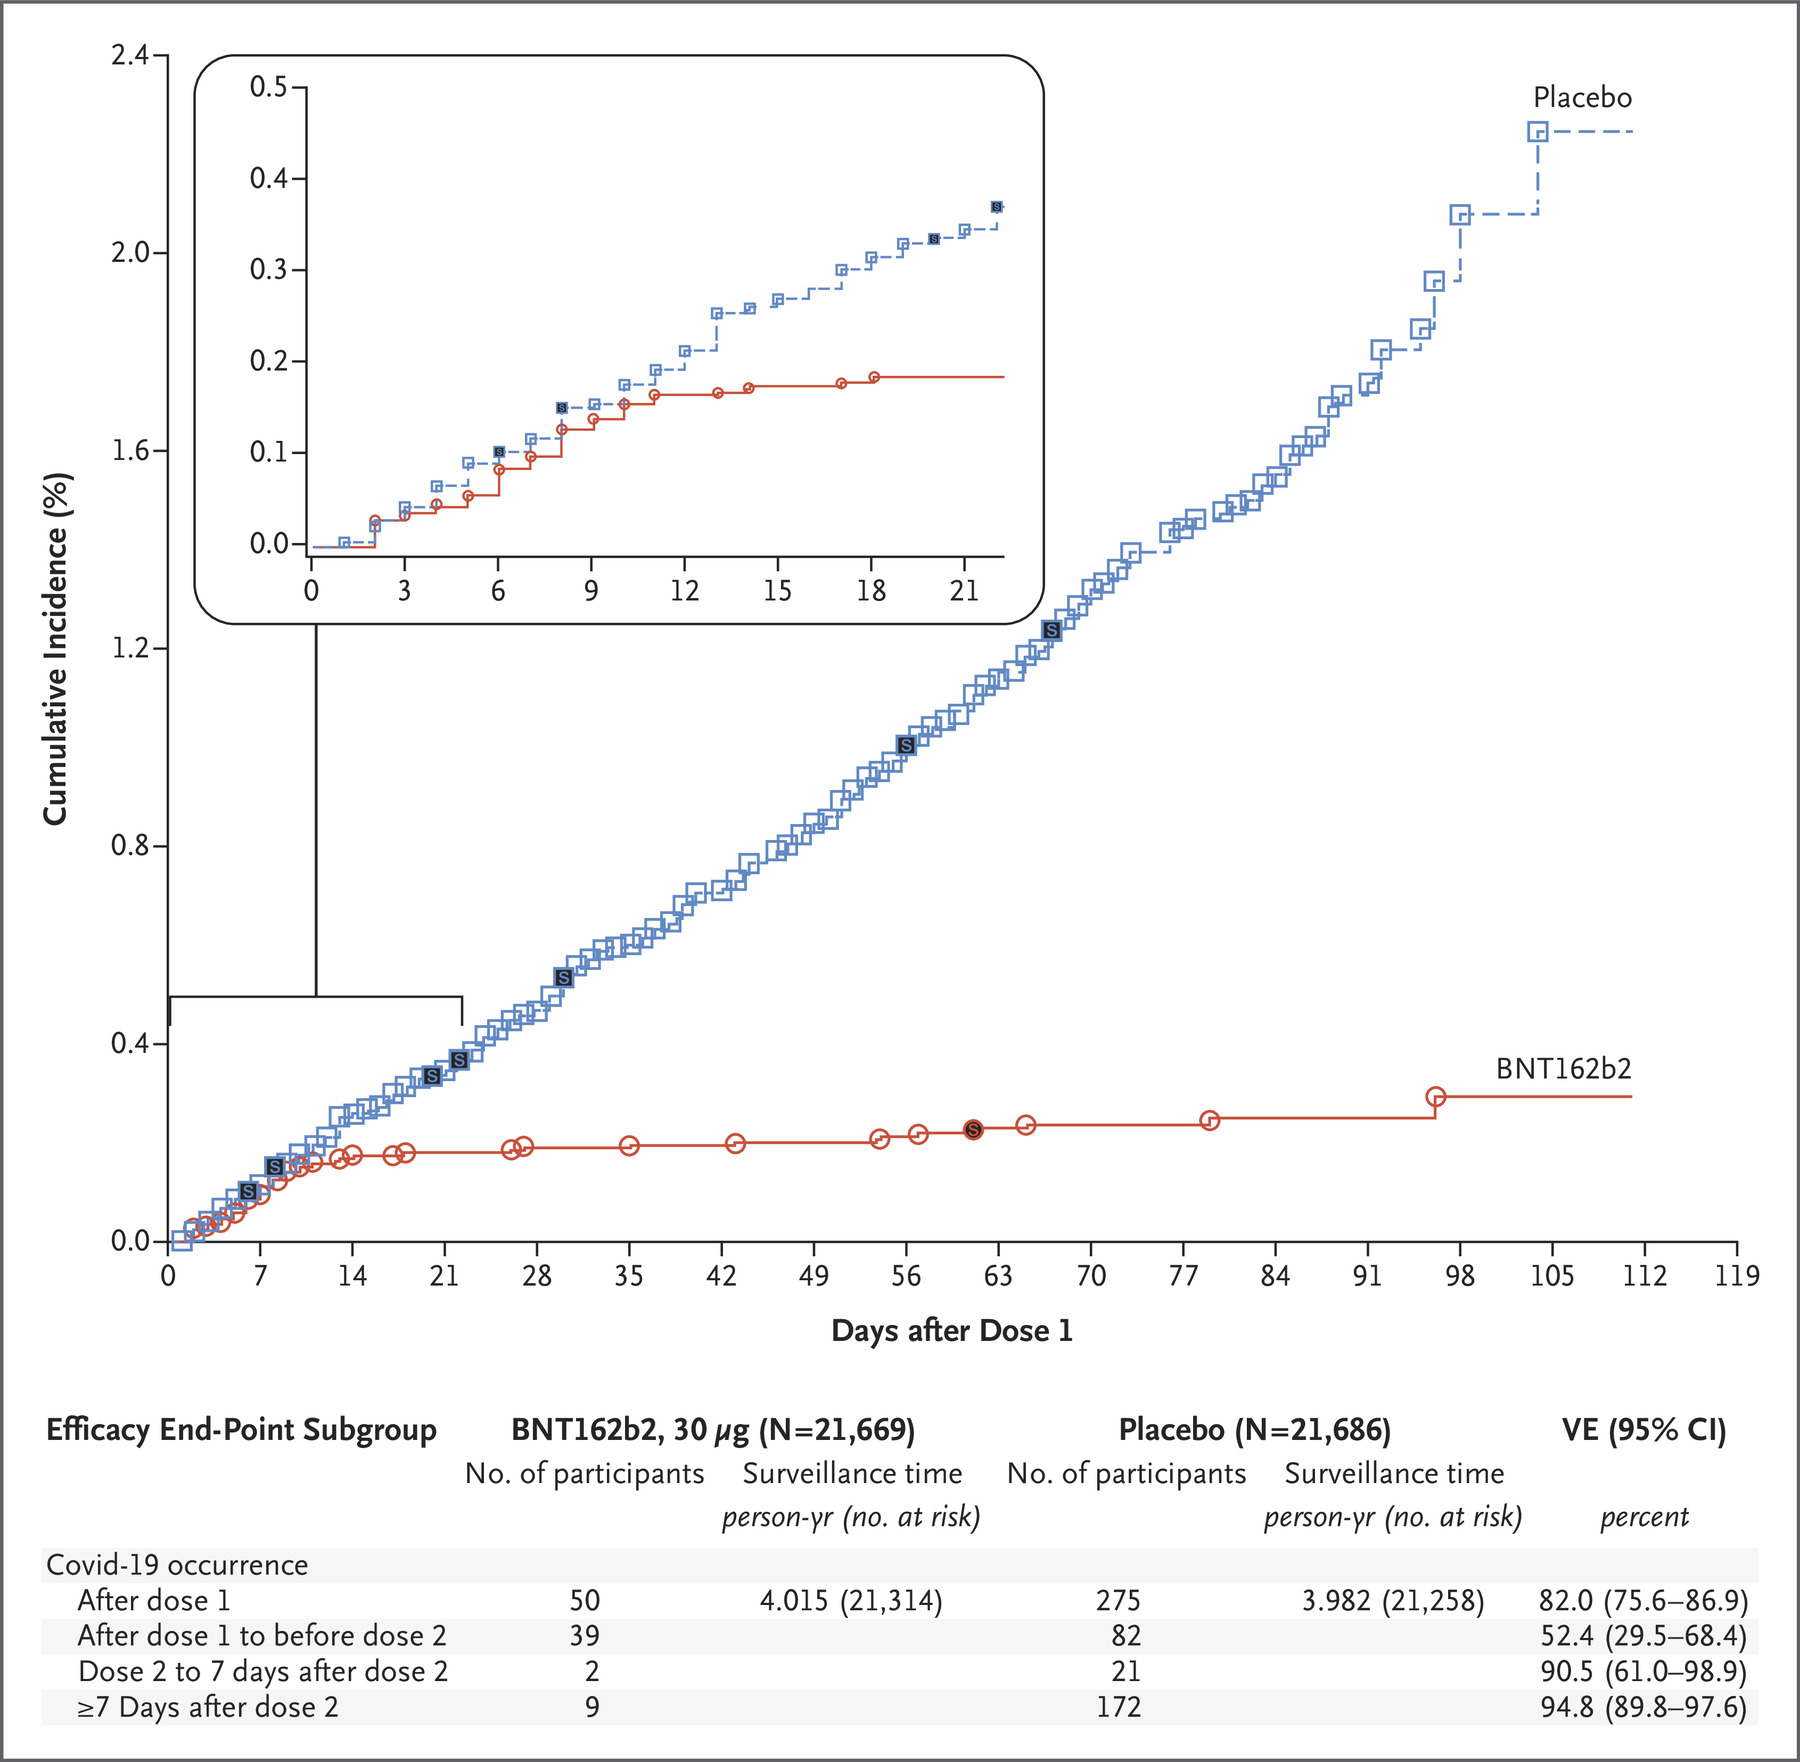
\includegraphics[width=\textwidth]{moderna_efficacy.jpeg}}
    \only<6>{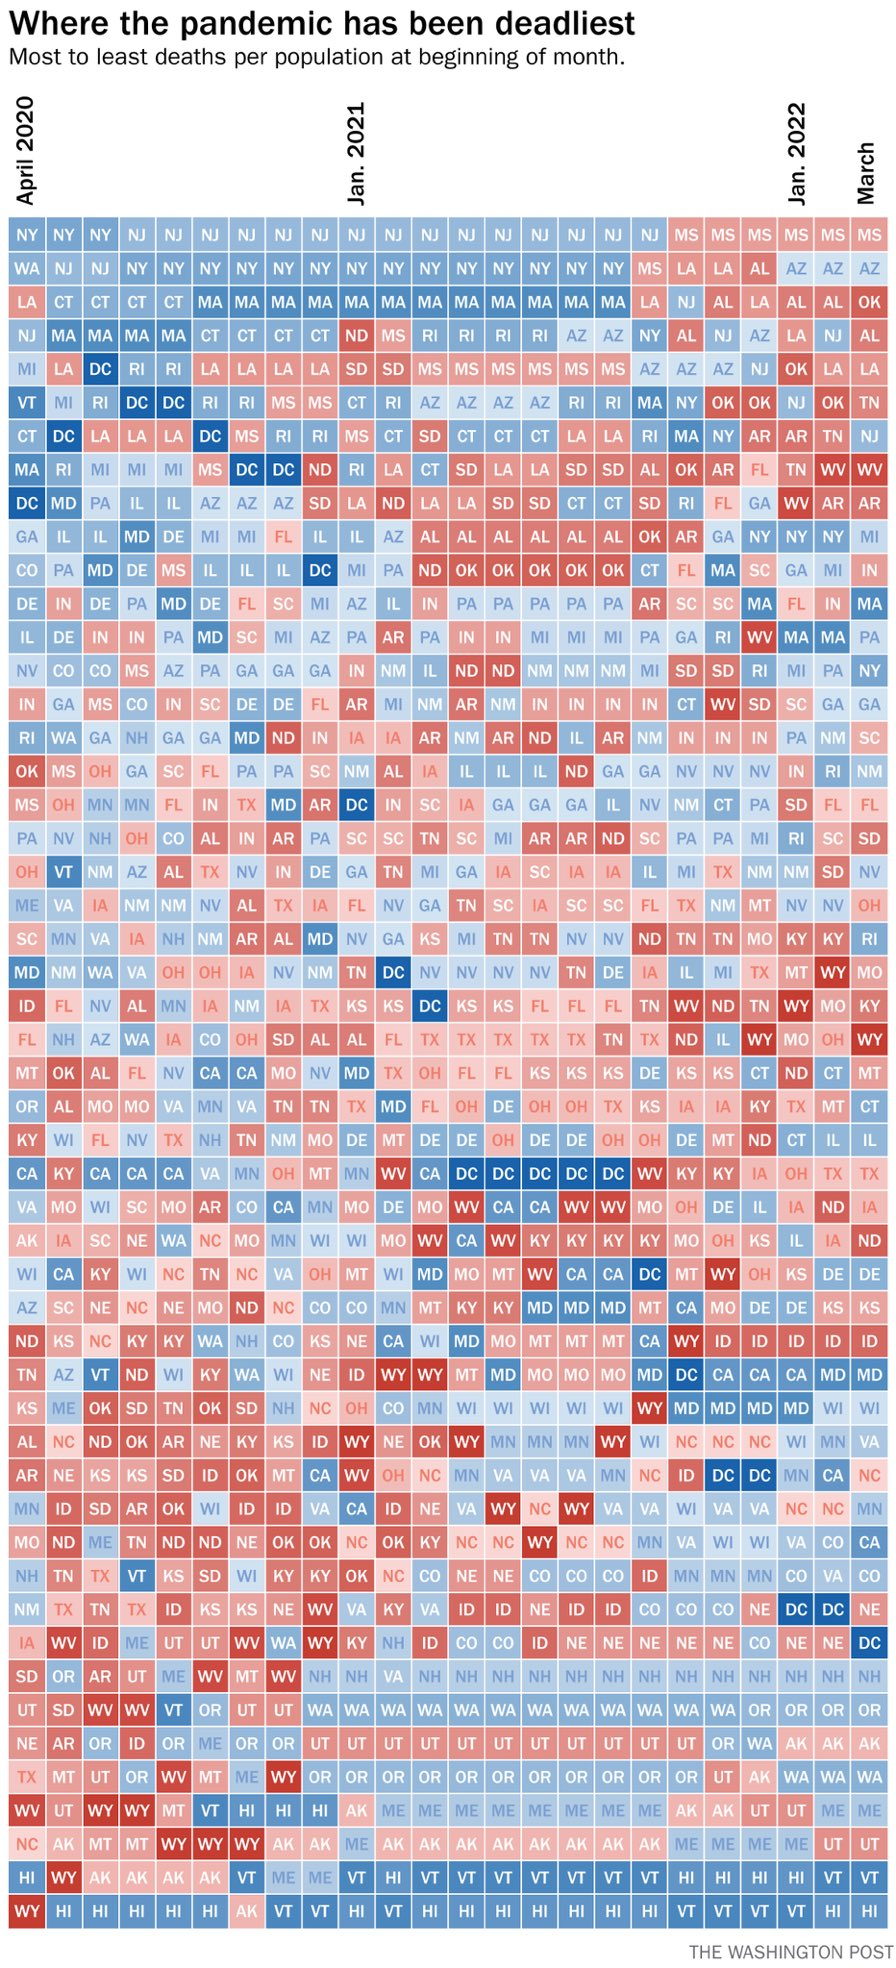
\includegraphics[height=.85\textheight]{wapo_pandemic_states.jpg}}
    \only<7>{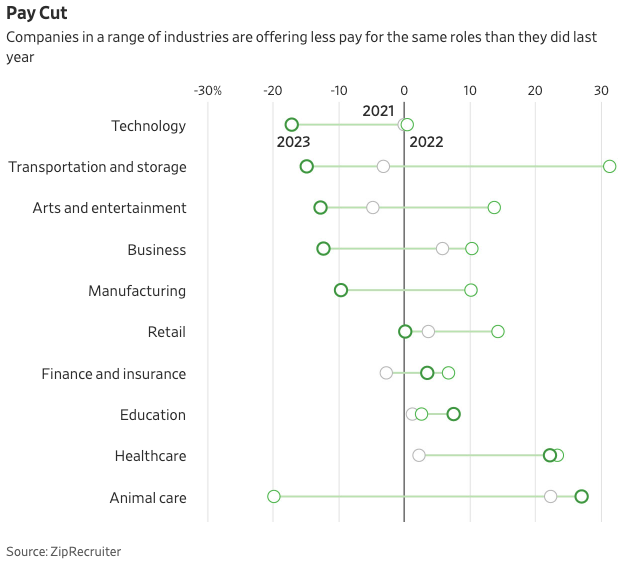
\includegraphics[width=\textwidth]{wsj_pay.png}}
    \only<8>{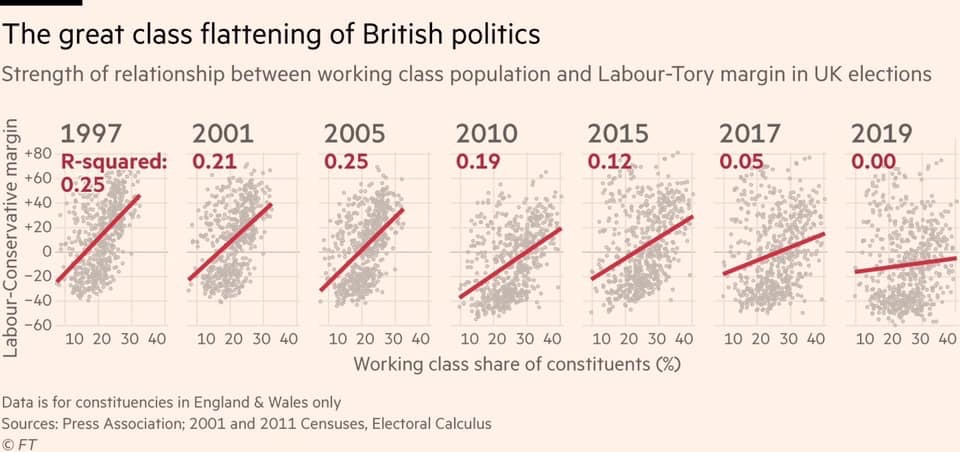
\includegraphics[width=\textwidth]{ft_britishpolit.JPG}}
    \only<9>{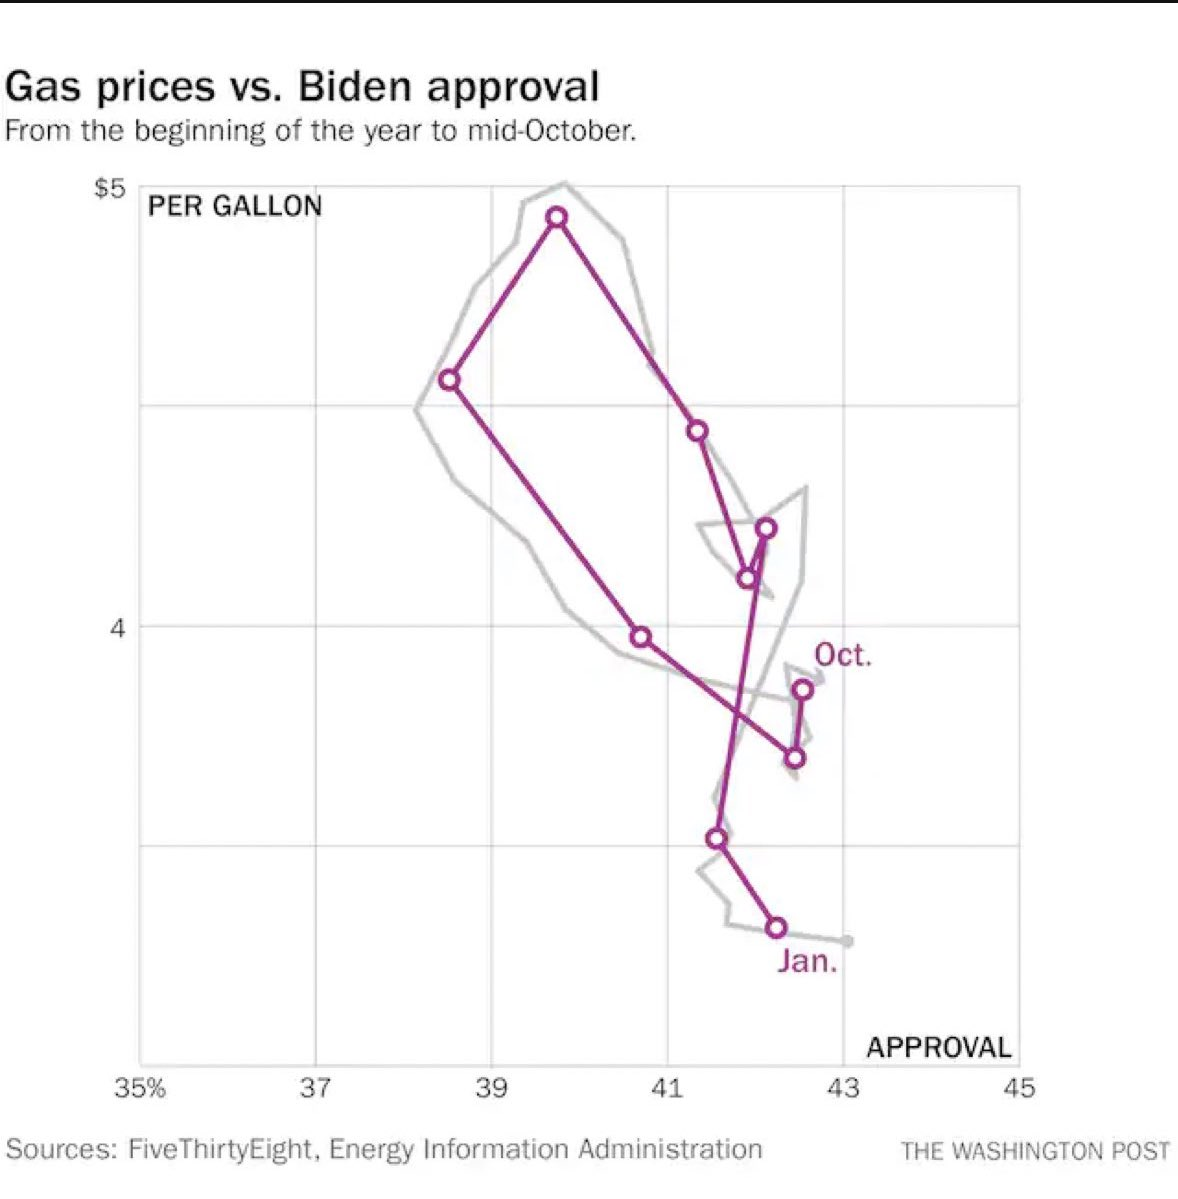
\includegraphics[width=\textwidth]{wapo_gas_prices.jpg}}
    \only<10>{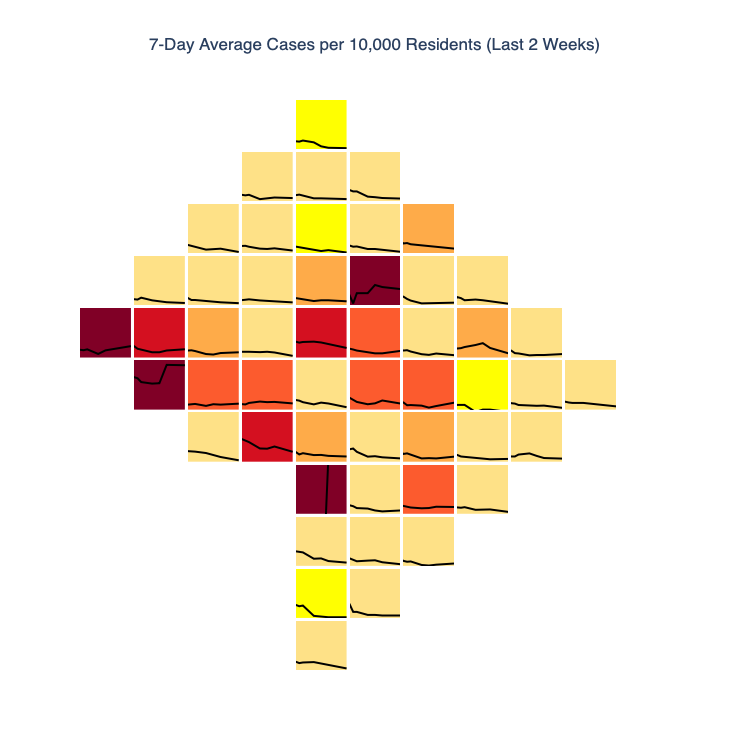
\includegraphics[width=\textwidth]{DC_covid.png}}
    \only<11>{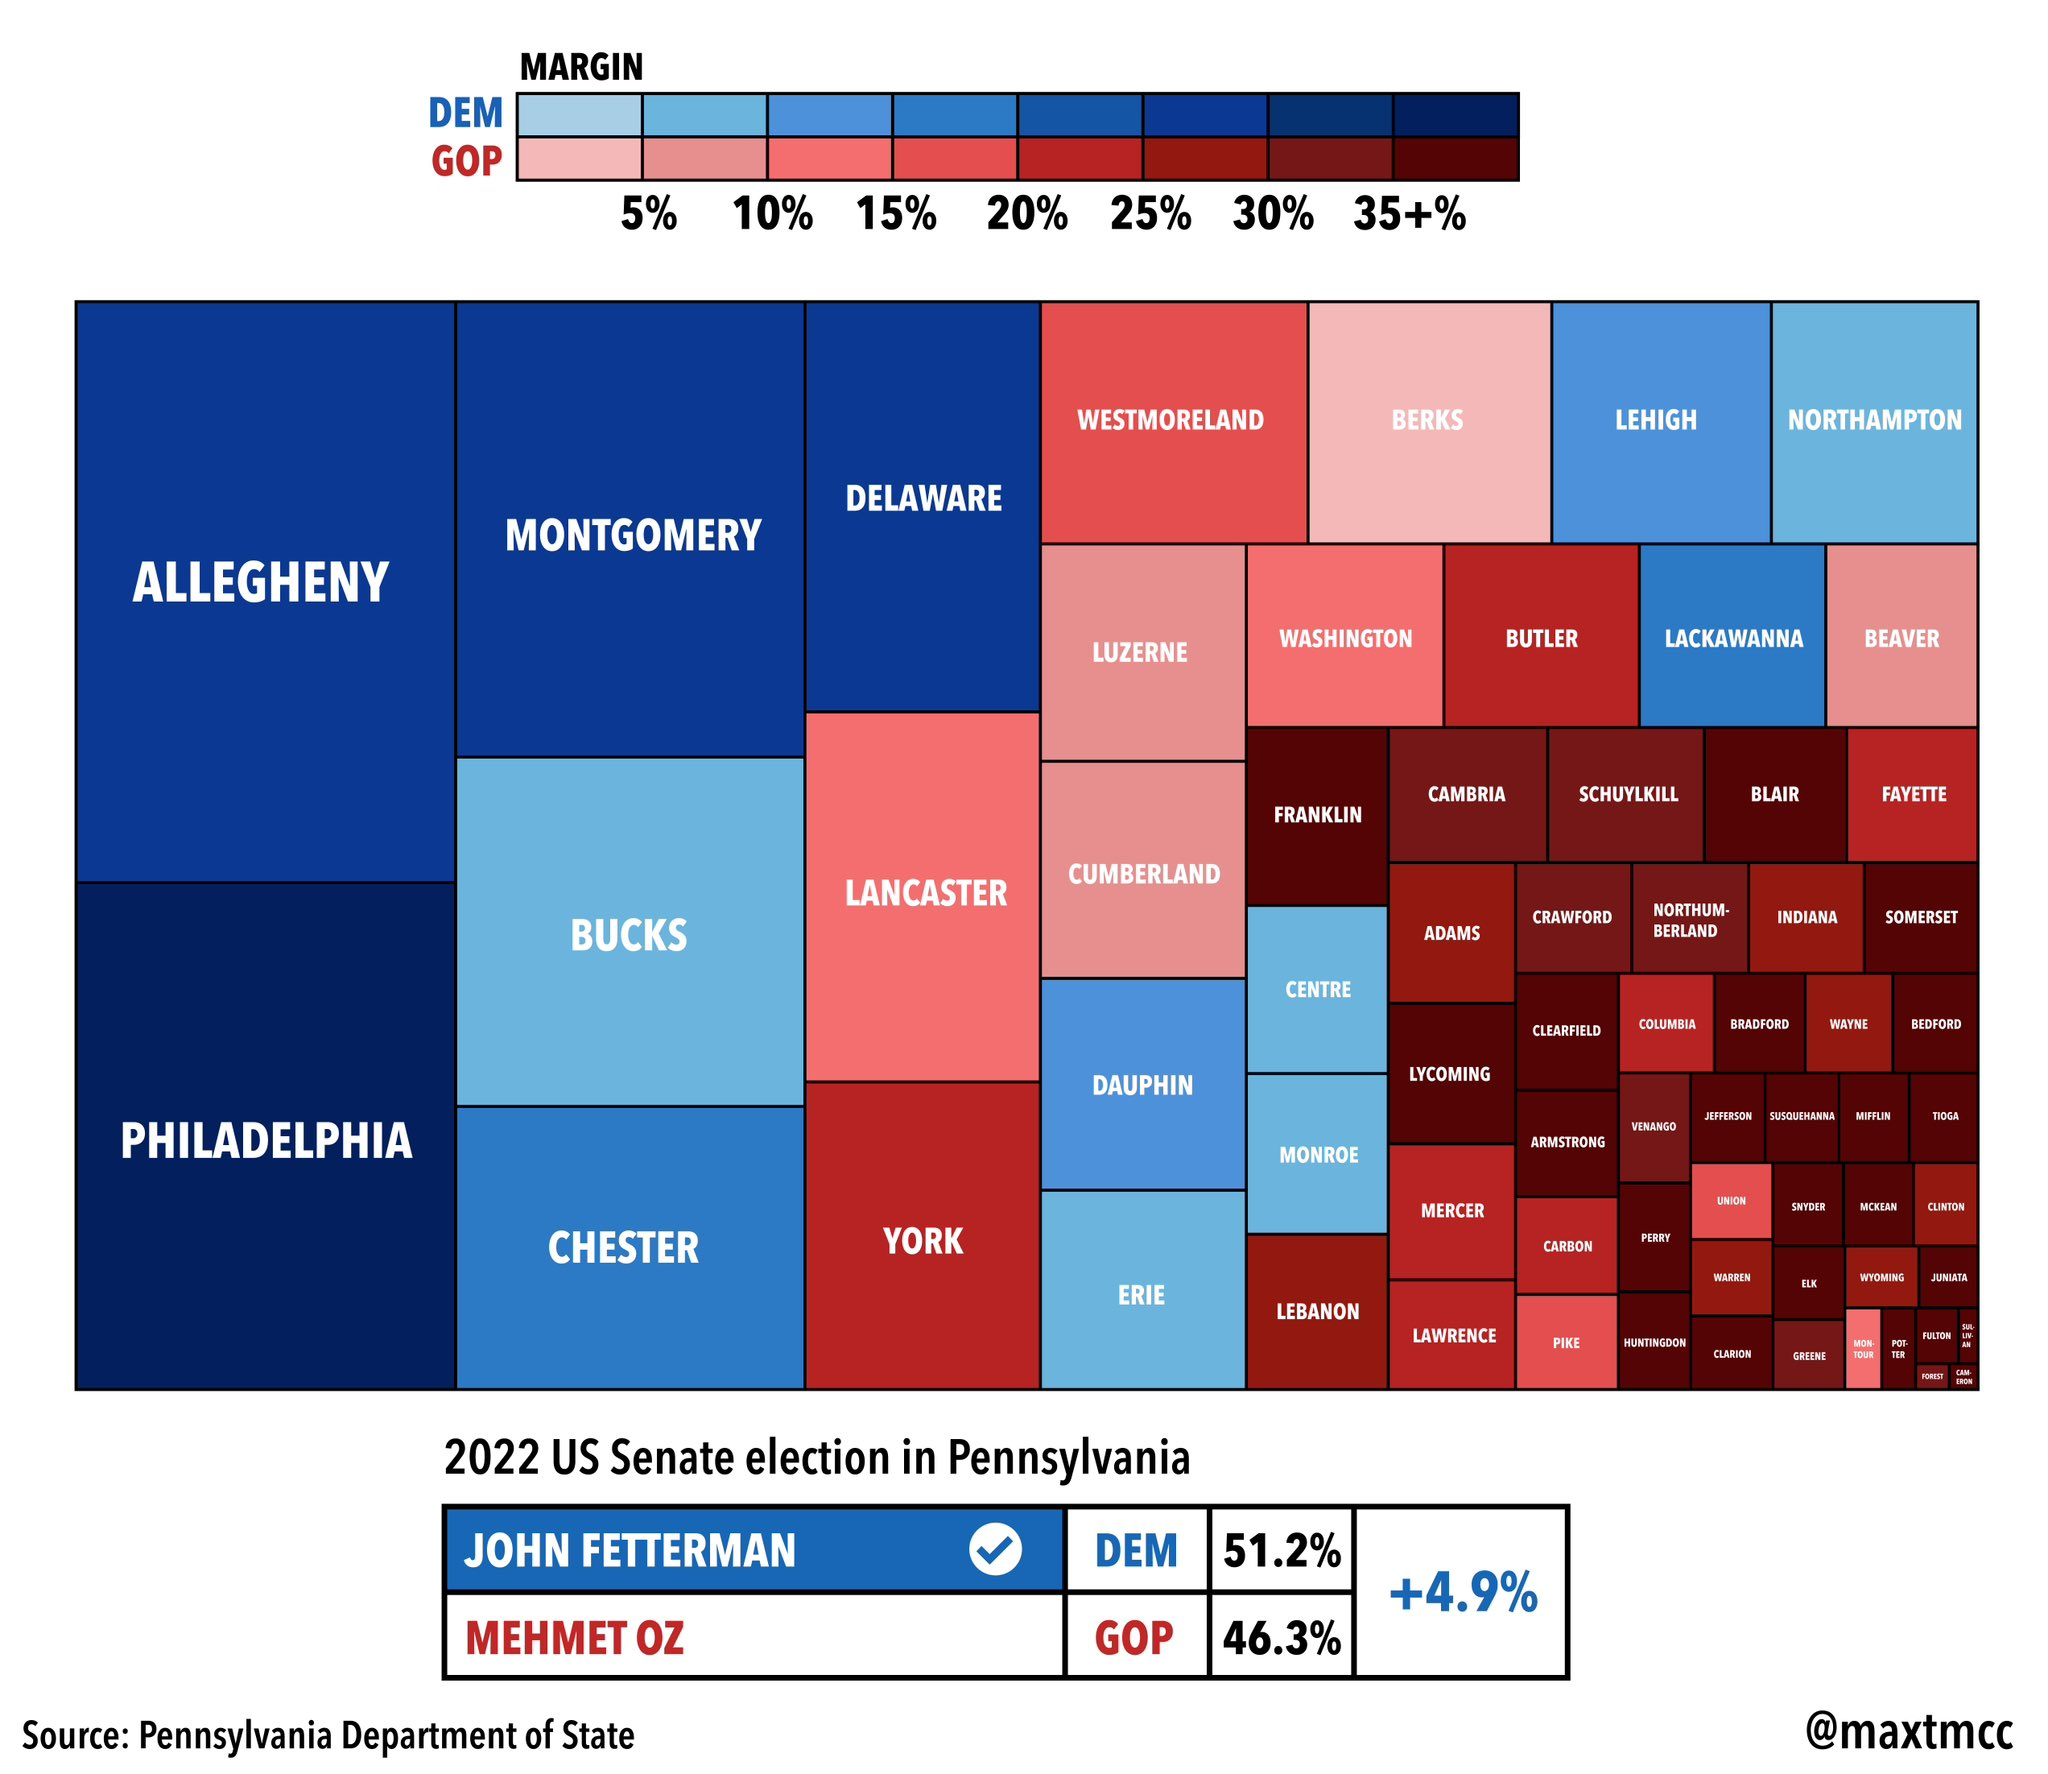
\includegraphics[width=\textwidth]{pa_sen_result.jpg}}
    \end{columns}
}
}

%%%%%%%%%%%%%%%%%%%%%%%%%%%%%%%%%%%%%%%%%%%%%%%%%%%%%%%%%%%%%%%%%%
\frame{\frametitle{Parts of a Graph}
    \centering
    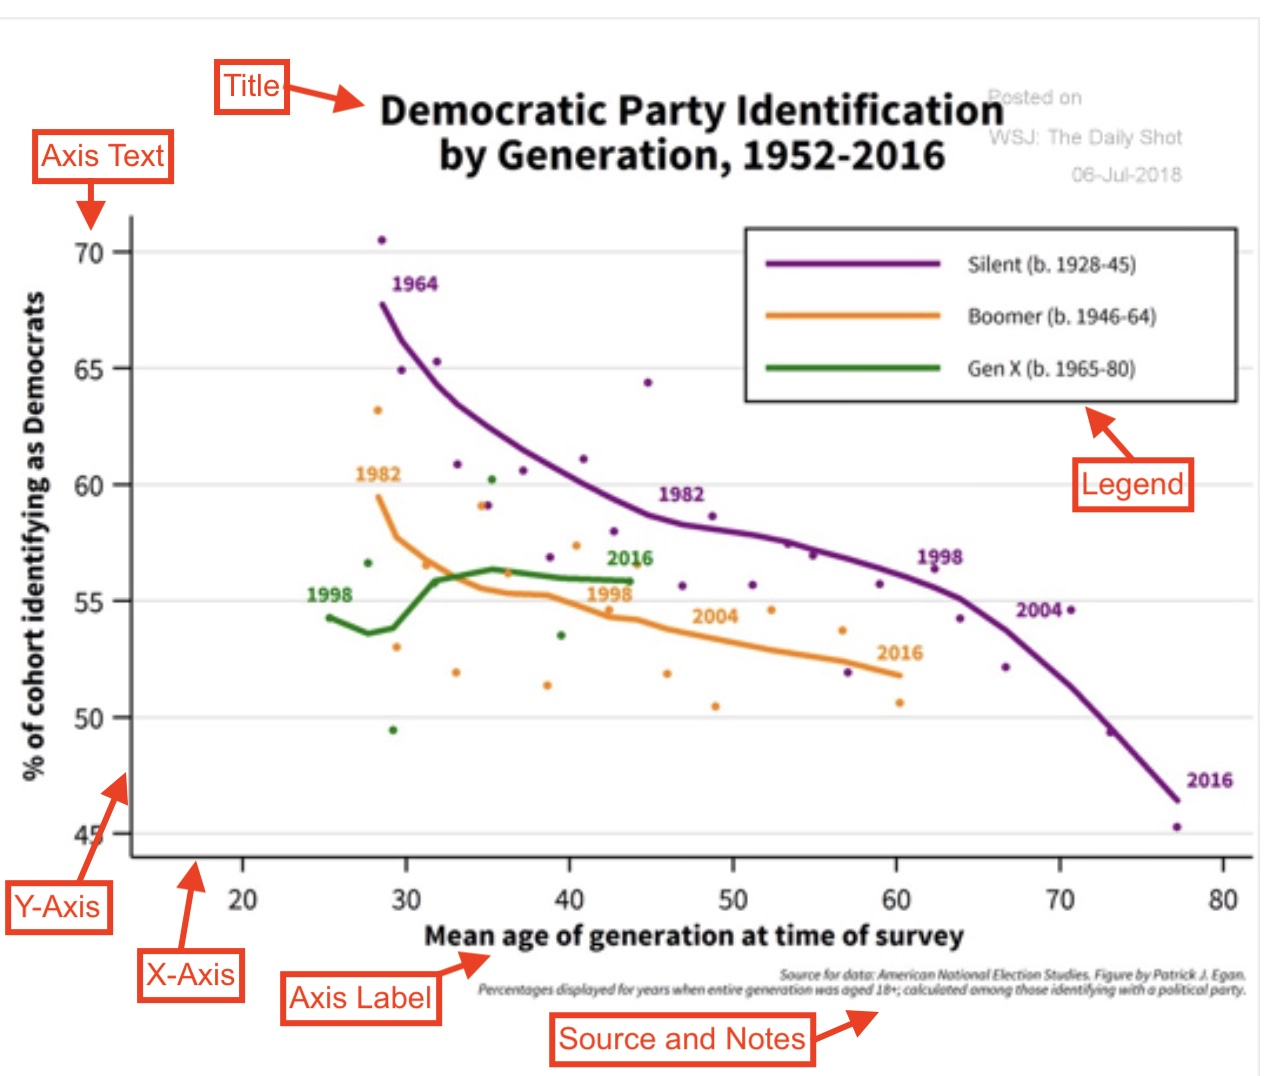
\includegraphics[width=.75\textwidth]{partsofgraph.jpg}
}

%%%%%%%%%%%%%%%%%%%%%%%%%%%%%%%%%%%%%%%%%%%%%%%%%%%%%%%%%%%%%%%%%%
\frame{\frametitle{Designing for Statistics}
\begin{columns}
\column{0.4\textwidth}
\begin{enumerate}[<+->]
        \item<1-> The main axis should start at 0
        \item<4-> The main axis should show the scale of the data
        \item<5-> There should be one x-axis and one y-axis
        \item<6-> Numbers get larger from bottom to top and left to right
        \item<8-> Trust ``the feeling behind our eyes'' (Joseph Williams)
        \item<10-> Pie charts should have no more than two slices
    \end{enumerate}
\column{0.6\textwidth}
\centering
\only<1>{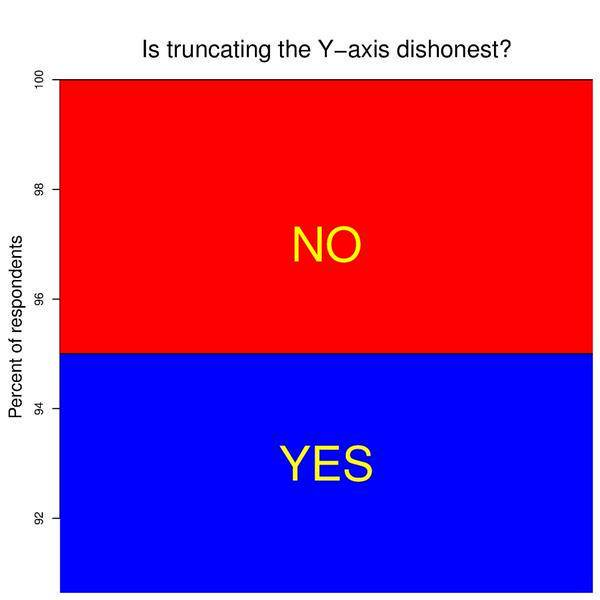
\includegraphics[width=\textwidth]{yaxis.jpeg}}
\only<2>{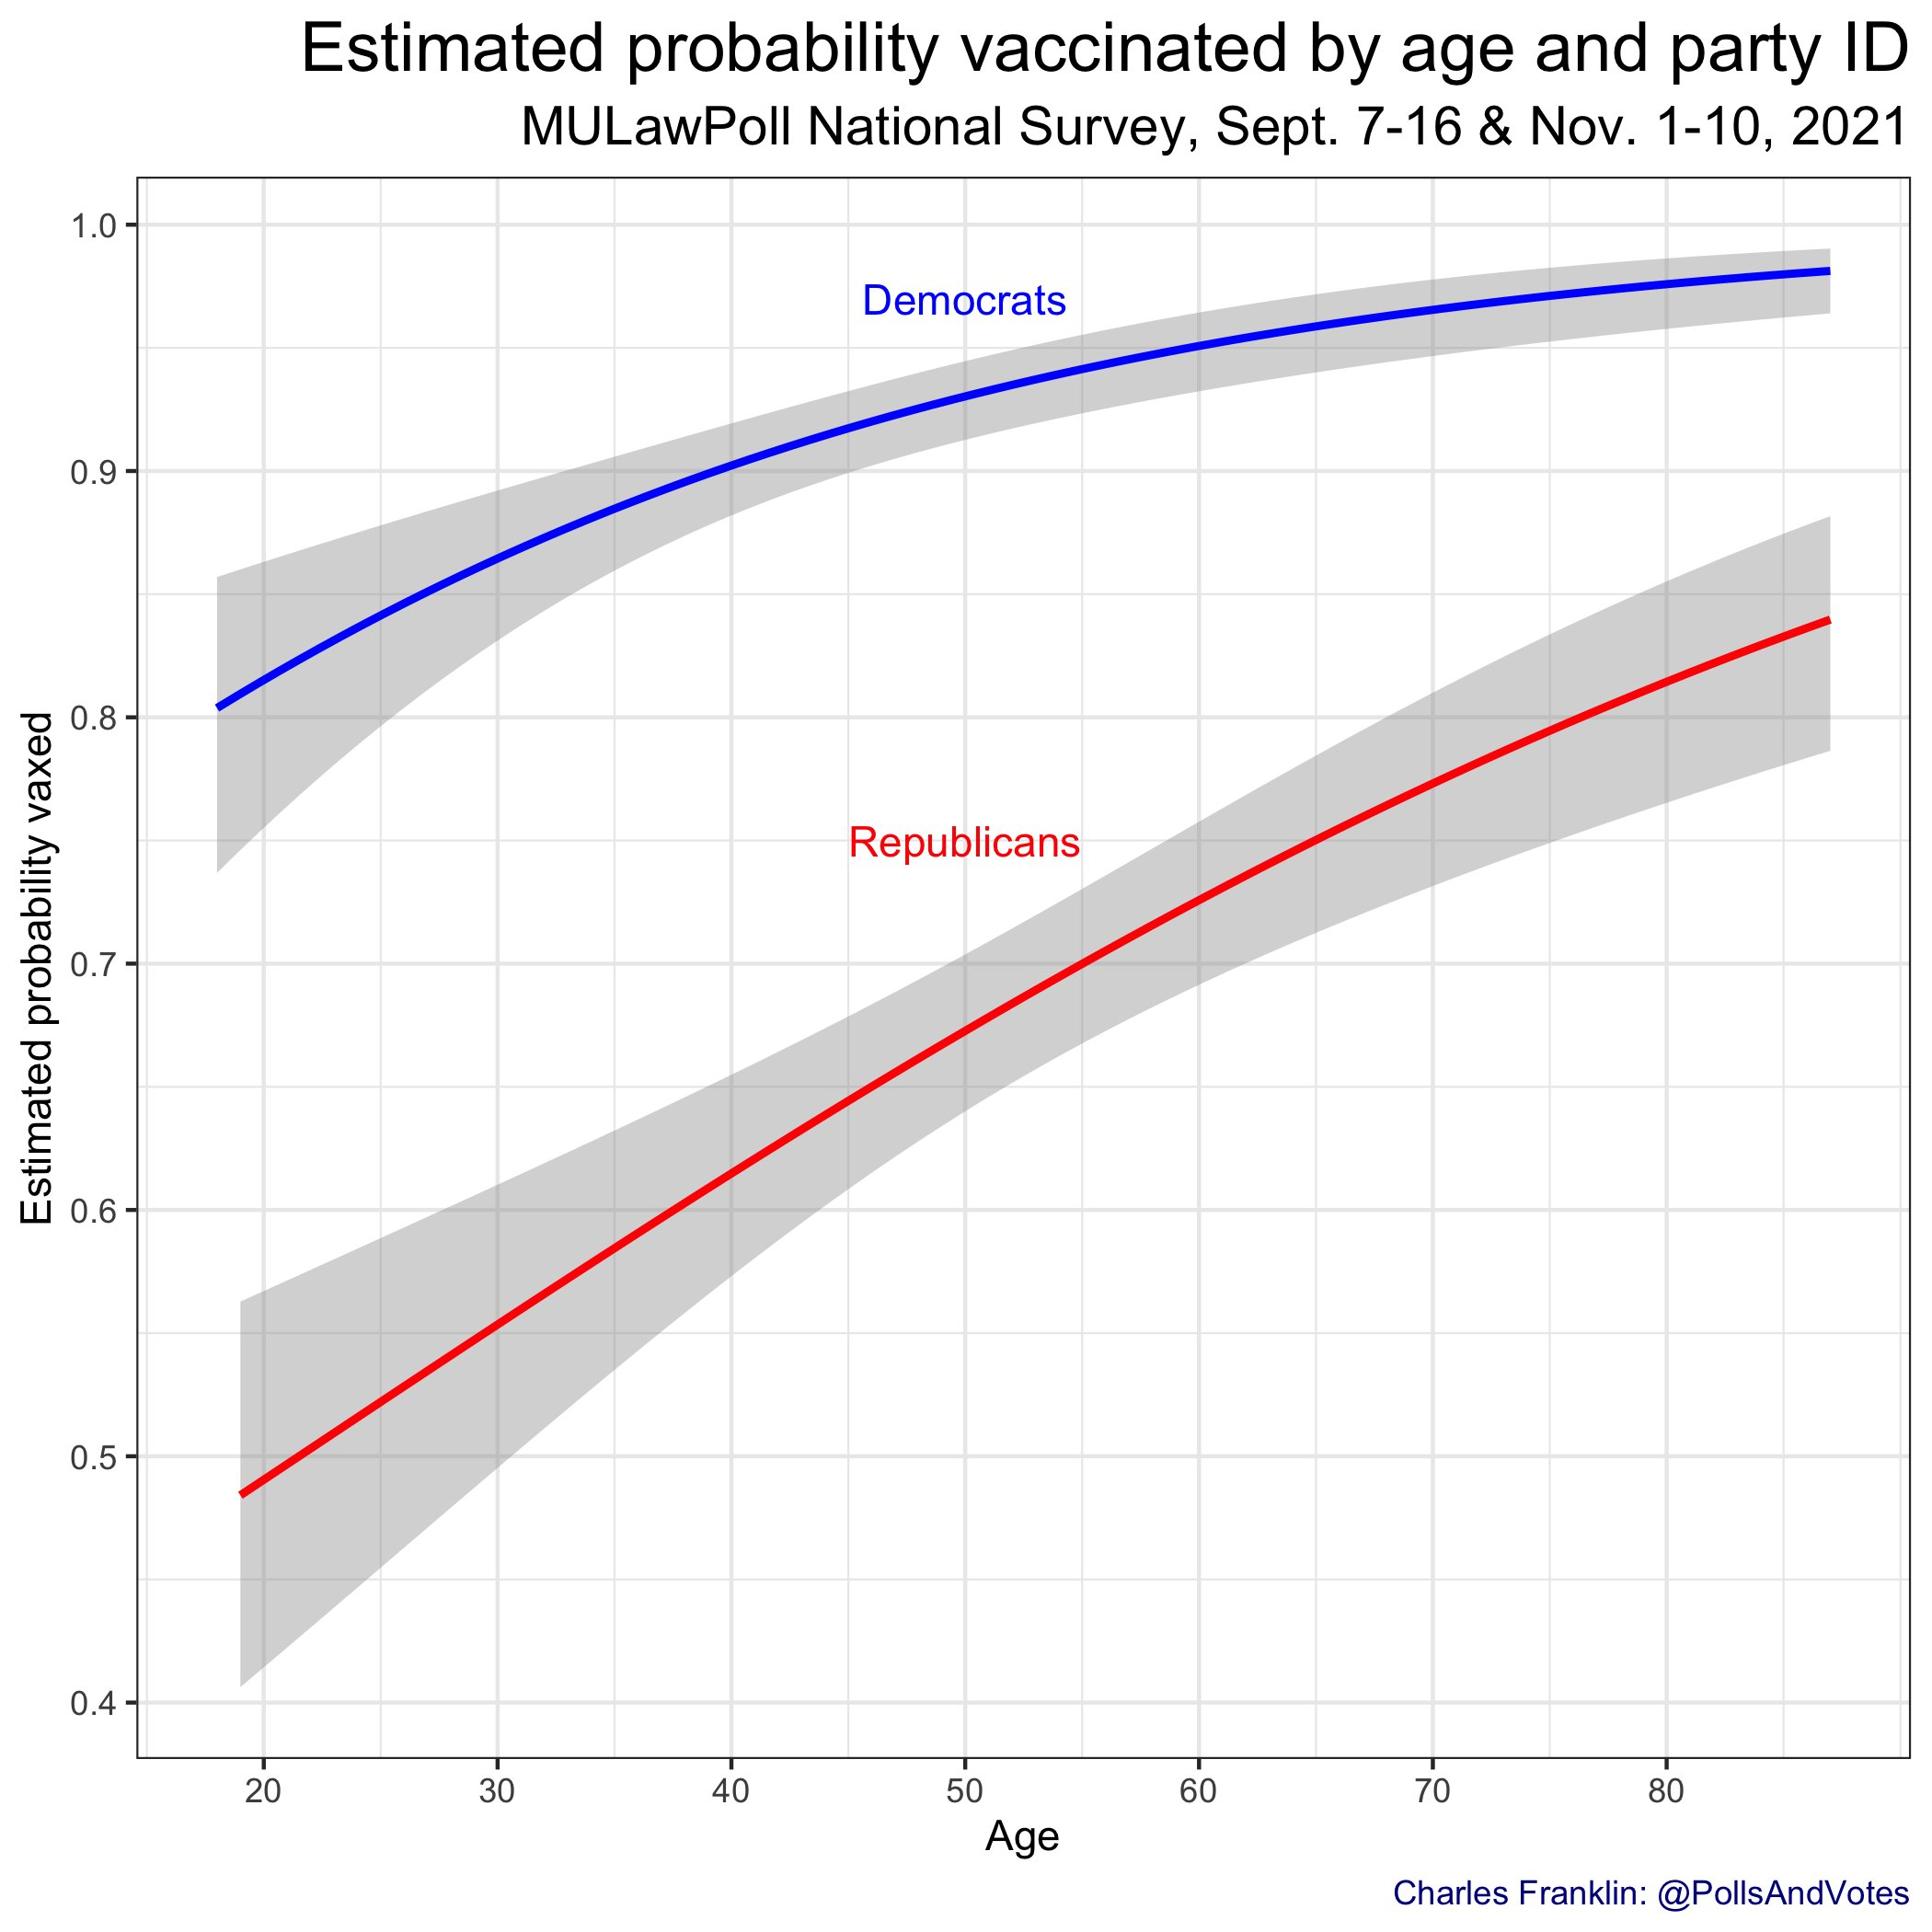
\includegraphics[width=\textwidth]{vaccine_take_up.jpg}}
\only<3>{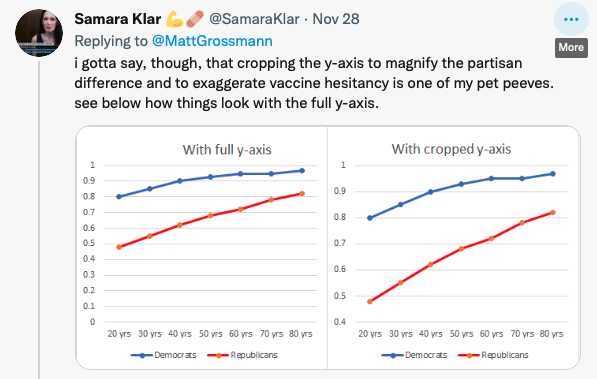
\includegraphics[width=\textwidth]{vaccine_take_up_response.png}}
\only<4>{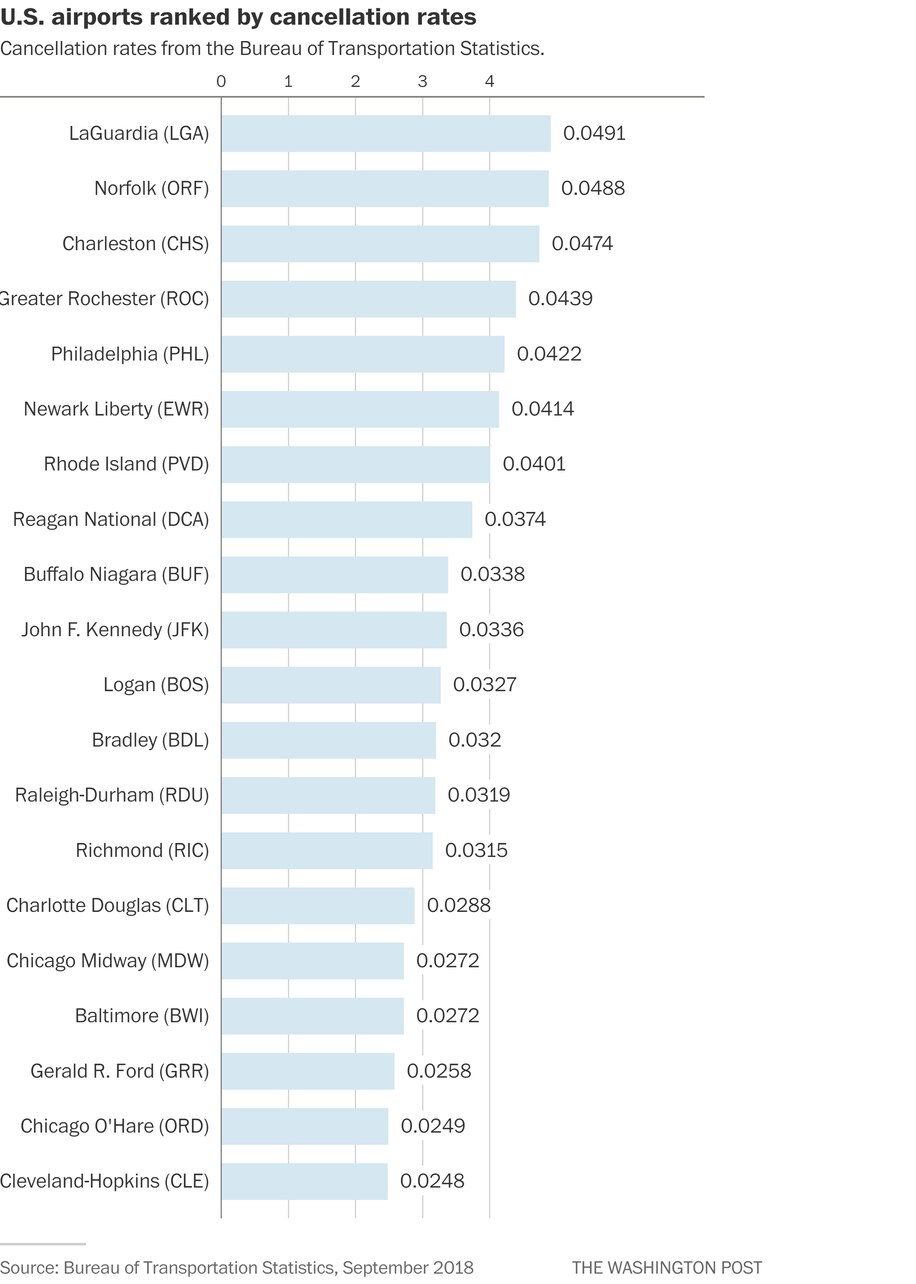
\includegraphics[height=.85\textheight]{xaxis.jpeg}}
\only<5>{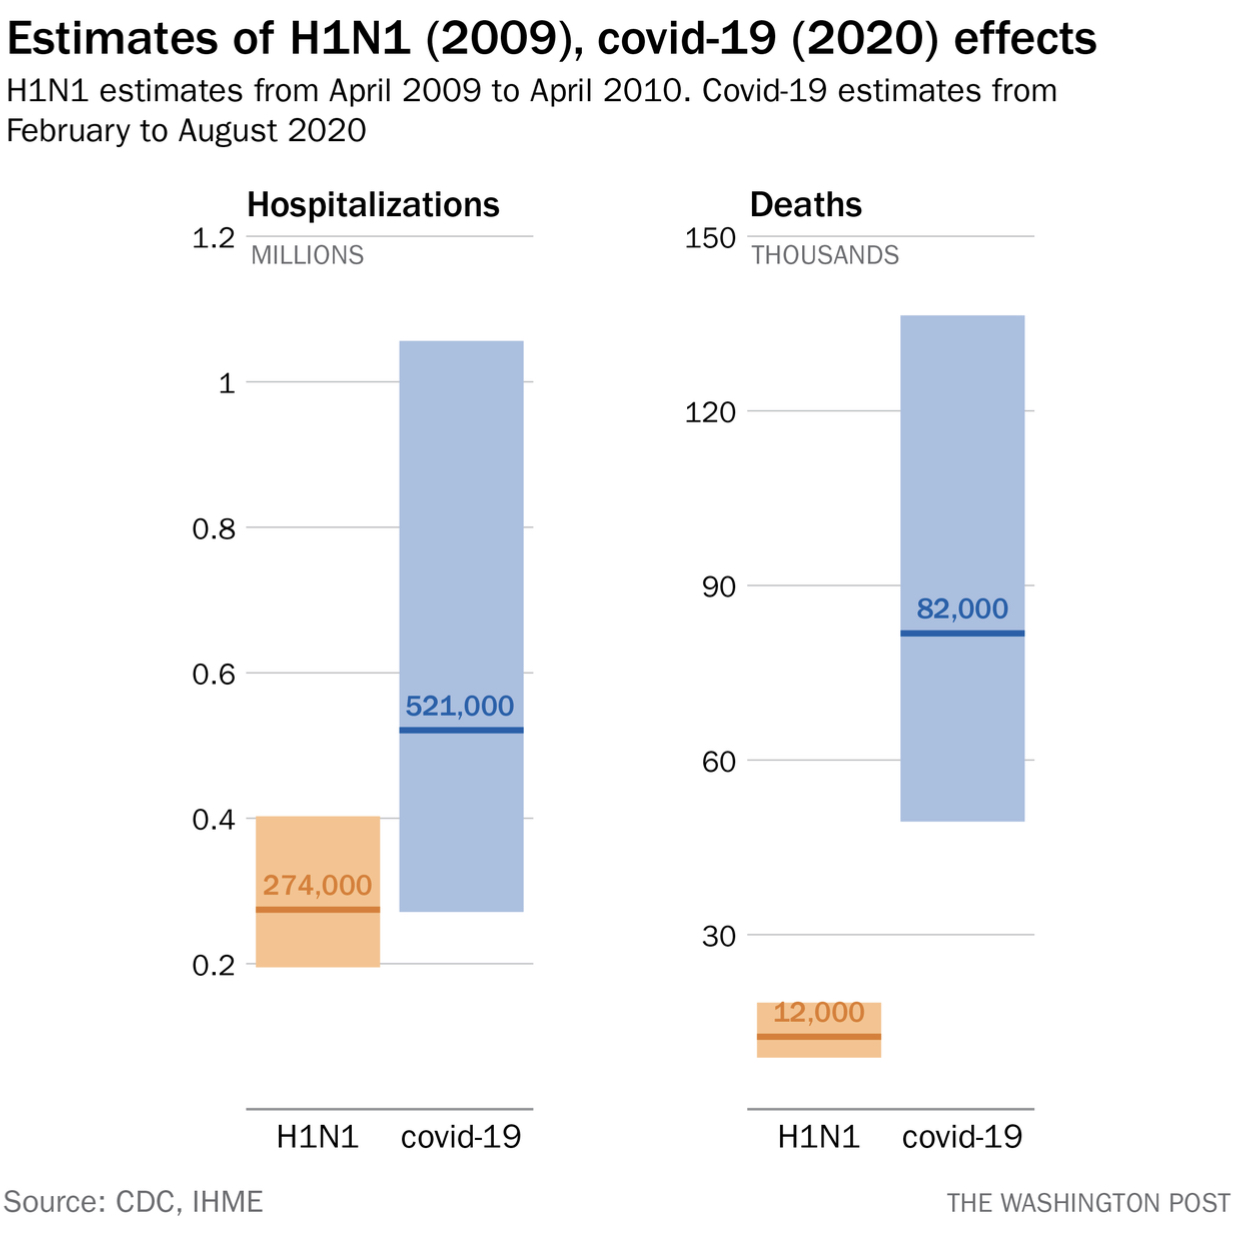
\includegraphics[width=\textwidth]{doubleyaxis.jpg}}
\only<6>{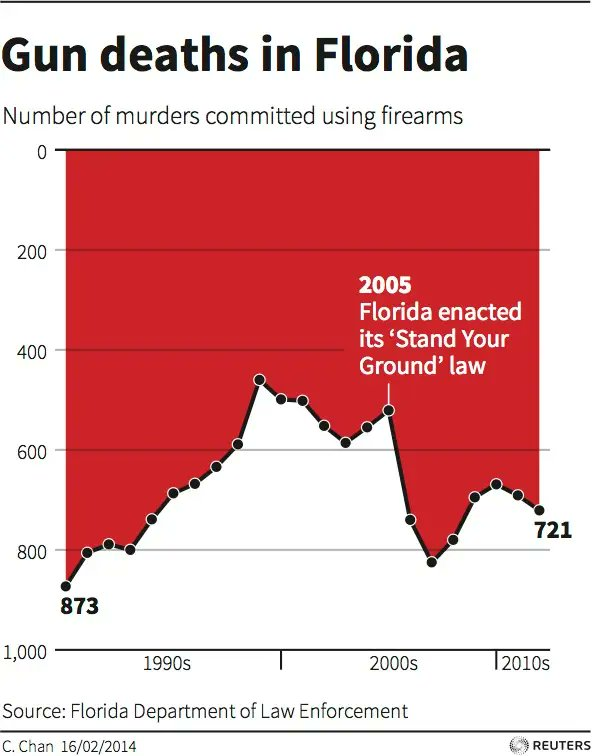
\includegraphics[height=.8\textheight]{reuters_guns.jpg}}
\only<7>{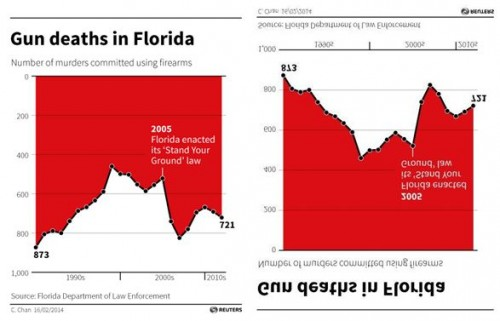
\includegraphics[width=\textwidth]{guns_flipped.jpeg}}
\only<8>{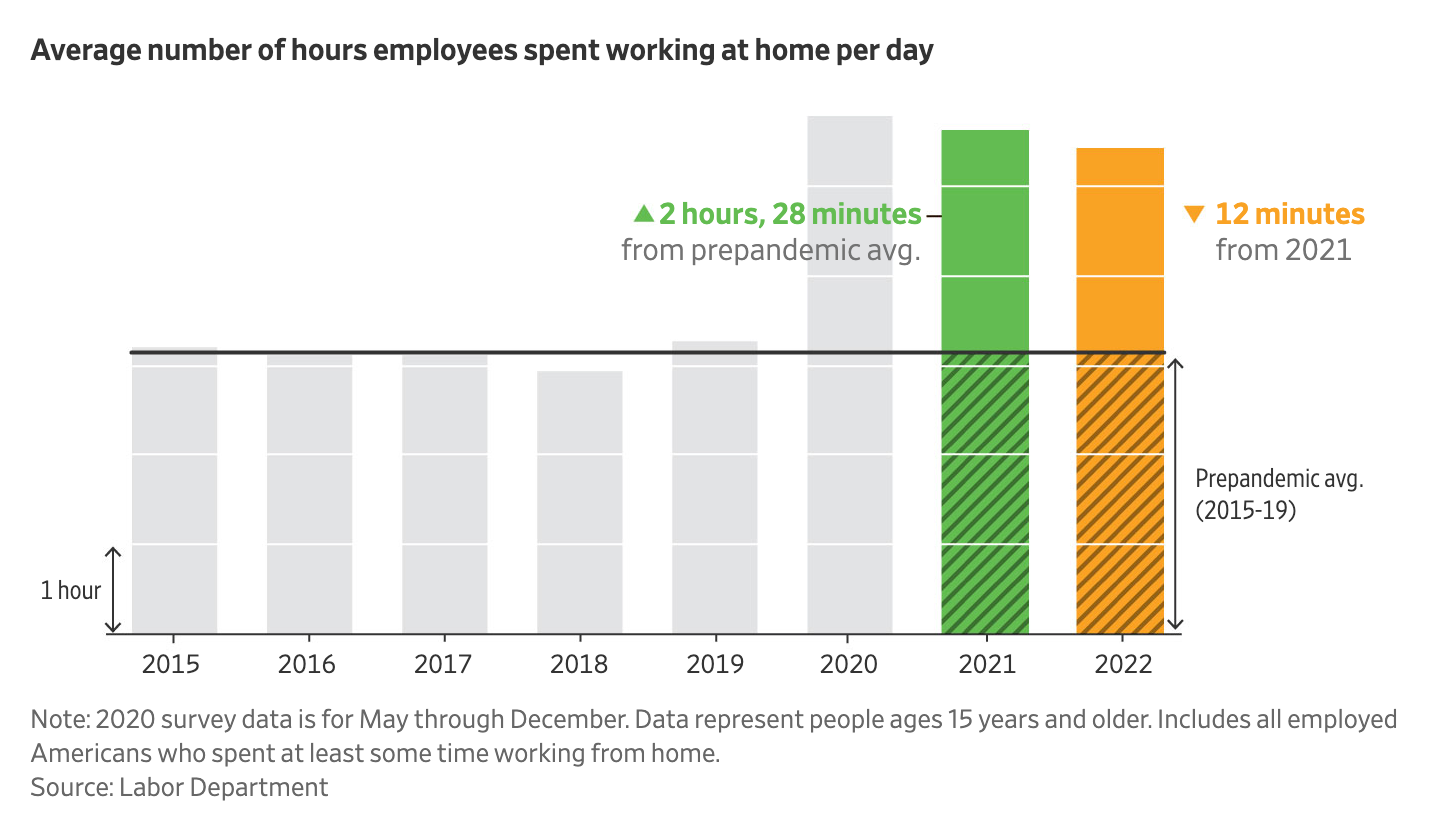
\includegraphics[width=\textwidth]{wsj_wfh.png}}
\only<9>{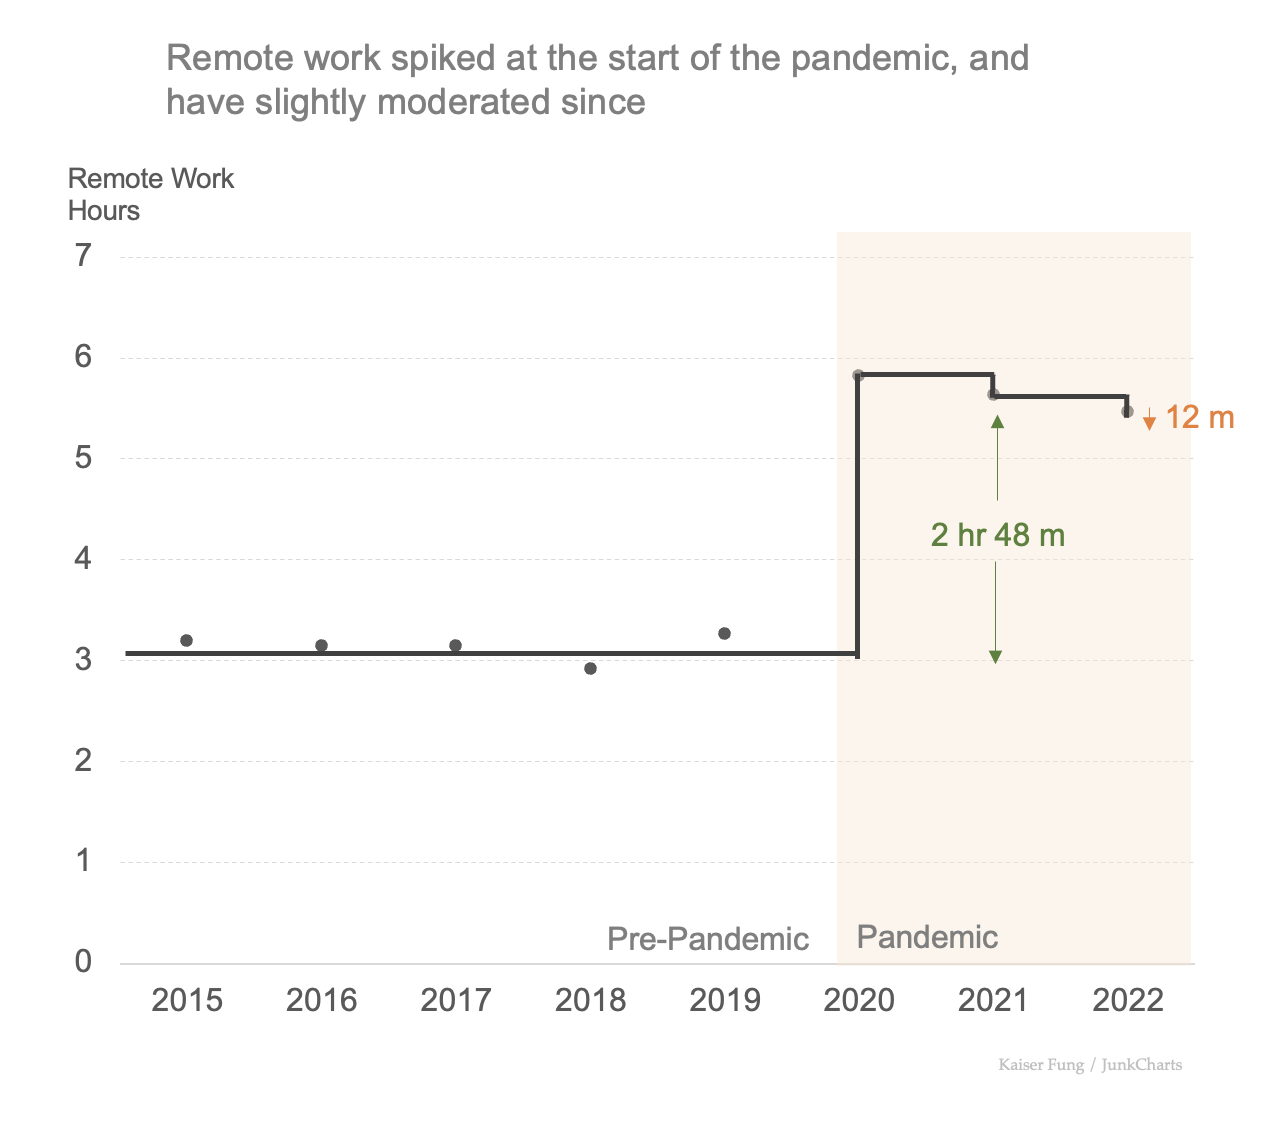
\includegraphics[width=\textwidth]{wfh_redesigned.png}}
\only<10>{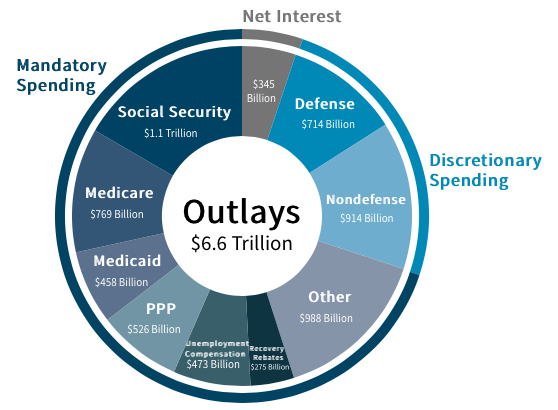
\includegraphics[width=\textwidth]{fedbudget2020.png}}
\end{columns}
}

%%%%%%%%%%%%%%%%%%%%%%%%%%%%%%%%%%%%%%%%%%%%%%%%%%%%%%%%%%%%%%%%%%
\frame{\frametitle{Evaluating a Graph}
\begin{columns}
\column{0.4\textwidth}
\begin{enumerate}
    \item Make a note of the first few things you see
    \item Make a note of the first idea that forms in your mind and then search for more
    \item Make notes on likes, dislikes, and wish-I-saws
    \item Find three things you'd change and briefly say why
\end{enumerate}
\column{0.5\textwidth}
\centering
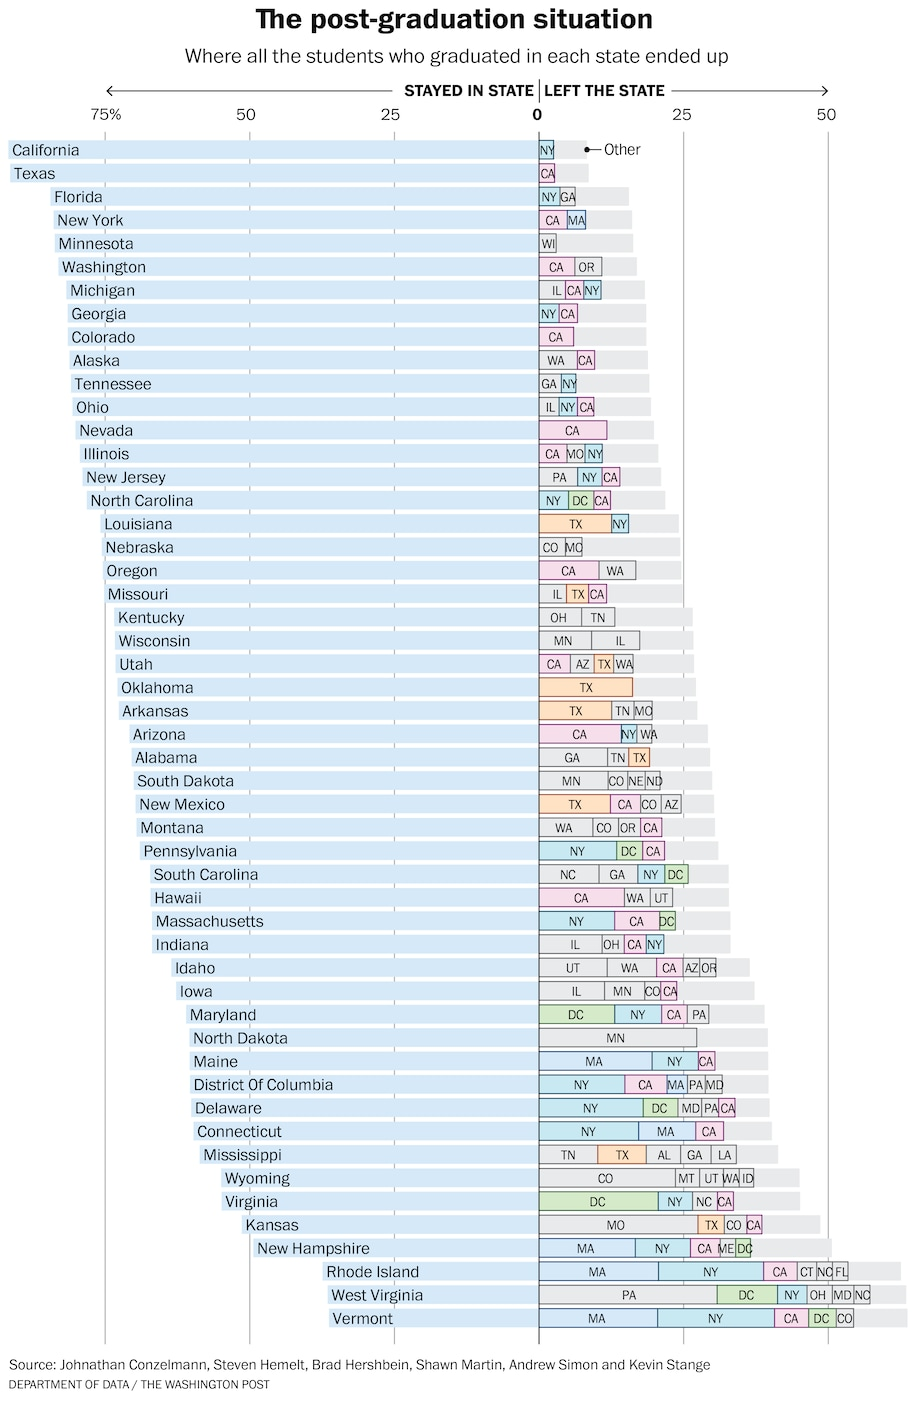
\includegraphics[height=.9\textheight]{wapo_graduates.jpg}
\end{columns}
}

\end{document}
